\documentclass[lettersize,journal]{IEEEtran}
%\usepackage{amsmath,amsfonts}
%\usepackage{algorithmic}
%\usepackage{algorithm}
\usepackage{array}
\usepackage[caption=false,font=normalsize,labelfont=sf,textfont=sf]{subfig}
\usepackage{textcomp}
\usepackage{stfloats}
\usepackage{url}
\usepackage{verbatim}
\usepackage{graphicx}
\usepackage{cite}
\hyphenation{op-tical net-works semi-conduc-tor IEEE-Xplore}
% updated with editorial comments 8/9/2021

% self package
\usepackage[algoruled,linesnumbered]{algorithm2e}
\usepackage{amsmath,amssymb,amsfonts}
\usepackage{graphicx}
\usepackage{subfloat}
\usepackage{tabularx}
%\usepackage{subfig}
\usepackage{multirow}
\usepackage{color,soul}
\usepackage{comment}
\usepackage{makecell}
% DIY
\usepackage{booktabs}
\usepackage{tabularx}
\usepackage{array}
\newcolumntype{L}{>{\raggedright\arraybackslash}X} % left-aligned X
\newcolumntype{R}{>{\raggedleft\arraybackslash}X}  % right-aligned X
\newcolumntype{C}{>{\centering\arraybackslash}X}   % center-aligned X
\newcolumntype{M}[1]{>{\centering\arraybackslash}m{#1}} % Centered vertical m column
\newcolumntype{P}[1]{>{\centering\arraybackslash}p{#1}}
% END
% end


\begin{document}

\title{R2F: A Practical DRL Framework to Optimize Fuzzing Strategy}

\author{IEEE Publication Technology,~\IEEEmembership{Staff,~IEEE,}
        % <-this % stops a space
\thanks{This paper was produced by the IEEE Publication Technology Group. They are in Piscataway, NJ.}% <-this % stops a space
\thanks{Manuscript received April 19, 2021; revised August 16, 2021.}}

% The paper headers
\markboth{Journal of \LaTeX\ Class Files,~Vol.~14, No.~8, August~2021}%
{Shell \MakeLowercase{\textit{et al.}}: A Sample Article Using IEEEtran.cls for IEEE Journals}

\IEEEpubid{0000--0000/00\$00.00~\copyright~2021 IEEE}
% Remember, if you use this you must call \IEEEpubidadjcol in the second
% column for its text to clear the IEEEpubid mark.

\maketitle

\begin{abstract}
	Coverage-guided fuzzing (CGF) is widely recognized as an effective approach for identifying software vulnerabilities and defects. Nevertheless, most existing research continues to depend on heuristic-based scheduling algorithms, which suffer from limited adaptivity to target programs, insufficient contextual modeling, and inadequate capacity to leverage prior experience. These constraints often lead to suboptimal exploration efficiency. While recent work has begun to investigate the use of deep reinforcement learning (DRL) to enhance fuzzing, such studies remain largely preliminary, focusing on feasibility rather than delivering comprehensive, deployable frameworks for real-world applications.
	
	To address these limitations, we propose ALFurther, a lightweight deep reinforcement learning framework designed to optimize fuzzing strategies in practical scenarios. First, we formulate the objective of CGF as an optimization problem, demonstrating that it can be modeled as a Markov Decision Process (MDP). We then leverage the Bellman optimality equation to derive optimal decisions for each fuzzing state, establishing a theoretical foundation for applying deep reinforcement learning to fuzzing scheduling. Next, we design and implement a DRL framework capable of continuously learning the exploration states of fuzzing, while generating optimized strategies for each sample with low computational overhead. Additionally, we introduce various effective methods to integrate this reinforcement learning framework into existing fuzzers seamlessly.
	
	We conduct empirical evaluations on the publicly available Unibench and Magma benchmark suites to demonstrate the effectiveness of ALFurther. Experimental results show that  ALFurther achieve the highest edge coverage in the most programs in Unibench tests, and could find most bugs in MAGMA benchmarks. Besides, ALFurther could increase coverage by up to 10.1\%, discover 2.6 more bugs, and reduce bug-triggering times by up to 15.3$\times$ compared to the baseline fuzzer. The ablation study demonstrated the average overhead loss could be controlled within 10\%. All These results validate the effectiveness and potential of deep reinforcement learning in practical fuzzing optimization scenarios.
\end{abstract}

\begin{IEEEkeywords}
Article submission, IEEE, IEEEtran, journal, \LaTeX, paper, template, typesetting.
\end{IEEEkeywords}

\section{Introduction}

Coverage-guided fuzzing (CGF) is one of the most widely used techniques for vulnerability discovery in practice \cite{zhuFuzzingSurveyRoadmap2022,huangBalanceSeedScheduling2023,liDeepLearningCoverageguided2022,boehmeFuzzingChallengesReflections2021}. Its primary objective is to maximize code coverage during execution, thereby ensuring that a broad range of execution paths are explored. Prior work has shown that higher coverage is positively correlated with the likelihood of discovering bugs \cite{bohmeReliabilityCoveragebasedFuzzer2022}. Consequently, CGF can be formulated as an optimization problem in which the objective function is to maximize code coverage within a given testing time.

One direction of fuzzing optimization is to adapt the fuzzing strategy to the current fuzzing state in order to enhance effectiveness. Numerous studies have explored heuristic-based methods for this purpose. For example, AFL~\cite{AmericanFuzzyLop} prioritizes the execution of seeds considered favored, while AFLFast~\cite{bohmeCoveragebasedGreyboxFuzzing2019} models the fuzzing process as a Markov chain and schedules seeds based on the rarity of the paths visited. Similarly, MOPT~\cite{lyuMOPTOptimizedMutation2019} formulates fuzzing optimization as a mutator scheduling problem and employs a swarm intelligence algorithm to determine the optimal probability distribution of mutators, thereby improving performance. However, heuristic-based fuzzing optimizations have several limitations. First, heuristics are essentially search methods that focus on finding feasible solutions without guaranteeing optimality. In fuzzing, this means they cannot ensure the highest possible reward for a given fuzzing state, thereby constraining effectiveness. Second, heuristic methods often rely on exhaustive search, which incurs additional time and resource costs, potentially reducing efficiency. For instance, MOPT employs a pilot fuzzing procedure to estimate the utility of each mutator using its swarm intelligence algorithm, which introduces extra overhead. These limitations have motivated researchers to explore more principled methods for optimizing fuzzing strategies.

With the advancement of reinforcement learning (RL) techniques, numerous studies have explored their application to coverage-guided fuzzing (CGF). RL-based fuzzing typically models the problem as a Markov Decision Process (MDP) and learns from past experience to derive an optimal policy for a given state. Based on Bellman optimality, RL can guarantee policy optimality after sufficient training. Moreover, by leveraging past experience, RL reduces unnecessary exploration and thereby decreases the cost of the search process. 

RL-based fuzzing can be broadly categorized into multi-armed bandit (MAB)-based and deep reinforcement learning (DRL)-based approaches. MAB-based fuzzing models the optimization problem as a bandit setting and applies bandit algorithms for decision-making. For example, EcoFuzz~\cite{yueEcoFuzzAdaptiveEnergysaving2020} formulates seed scheduling as an adversarial MAB problem and implements an adaptive scheduler to balance exploration and exploitation. SeamFuzz~\cite{leeLearningSeedadaptiveMutation2023} clusters seeds into groups based on their characteristics and employs Thompson Sampling to identify the optimal mutation probability distribution for each group.

While MAB-based approaches demonstrate the promise of RL, their linear modeling capacity restricts expressiveness in complex fuzzing scenarios\cite{cutkoskyDynamicBalancingModel2021}. In contrast, DRL-based fuzzing employs neural networks (NNs) to model fuzzing states and predict optimal policies through learning. Owing to the fitting capacity of NNs, DRL-based approaches provide stronger modeling and prediction capabilities compared to the linear modeling used in MAB-based methods, thereby offering greater potential for improving fuzzing performance. For instance, Böttinger et al.~\cite{bottingerDeepReinforcementFuzzing2018} were the first to model fuzzing as an MDP and adopt a Deep Q-Network to predict the mutator probability distribution given input bytes as the state. RainFuzz~\cite{binosiRainfuzzReinforcementlearningDriven2023} extended this direction by taking seed bytes as input to train PPO and predict mutation positions. In addition, several other studies~\cite{gongDRLFCfuzzerFuzzingDeepReinforcementLearning2022,jeonDrPathFinderHybrid2022,liangRLFDirectedFuzzing2022,liuXRLFuzzFuzzingBinaries2024} have demonstrated the feasibility of RL for fuzzing optimization through proof-of-concept experiments. Together, these pioneering works provided valuable early evidence for the feasibility of DRL-based fuzzing optimization, laying the groundwork for subsequent advances.

% Limitation
% Effectivness of DRL-based fuzzing has not been addressed: NN is black-box, without explanation, many will doubt the actual effect.
% No comprehensive state and action modeling, thereby limit the DRL-based fuzzing effectiveness. (example, Deep Reinforcement Fuzzing, RainFuzz)
% There are many practical problems in implementing DRL on fuzzing, while the current studies only focuing on validate the feasibility while not invesigate the implementation issues. For example: DRL Trainig, IPC, Resource allocation, etc.
However, in contrast to the successful application of DRL in other domains~\cite{zhaoSurveyRecentAdvancements2024,tangDeepReinforcementLearning2025,silverMasteringChessShogi2017} its apparent compatibility with fuzzing, DRL-based fuzzing remains far from practical deployment in real-world scenarios, thereby hindering progress in this direction. We summarize the limitations of current DRL-based fuzzing in the following three points.

Firstly, the effectiveness of DRL-based fuzzing has not been convincingly demonstrated. Prior work~\cite{bottingerDeepReinforcementFuzzing2018} formulated fuzzing as an MDP and applied DRL directly, but without explaining why this formulation should lead to effective strategies in practice. Moreover, since neural networks operate as black-box models, their learned policies are difficult to interpret, raising doubts about whether they truly capture the underlying dynamics of fuzzing. To address this gap, a theoretical foundation is necessary to show that DRL can obtain optimal fuzzing strategies in principal, which would be a foundation we establish in this paper.

Secondly, current DRL-based fuzzing methods have not fully leveraged the rich information available during fuzzing or designed integrated strategies to guide the process. Most studies rely on narrow state representations (e.g., static byte arrays of test cases) while overlooking runtime feedback such as execution coverage or path novelty. Likewise, they typically restrict actions to a single strategy — for instance, either mutator probability distributions~\cite{bottingerDeepReinforcementFuzzing2018,gongDRLFCfuzzerFuzzingDeepReinforcementLearning2022} or mutation positions~\cite{binosiRainfuzzReinforcementlearningDriven2023} — rather than combining multiple strategies. Such simplified modeling underutilizes the representational capability of neural networks, which are designed to capture complex, high-dimensional relationships. As a result, the potential benefits of DRL for fuzzing are diminished, since the agent cannot learn or exploit the richer dynamics of the fuzzing process.

Finally, several challenges in practical implementation remain unresolved. DRL requires a complex training pipeline, encompassing sample generation, training workflows, and policy interactions. Typically, a DRL workflow involves repeated trials on a single target: the model is trained multiple times on collected samples and then applied to the same target to achieve optimal performance. In contrast, fuzzing is an open-ended exploration process with no clear termination, meaning that the traditional DRL workflow cannot be applied directly, and an online learning approach is necessary. Moreover, fuzzing demands high I/O throughput to sustain massive test executions, imposing strict requirements on real-time interaction with the DRL agent. Unlike simulation environments, which provide standardized APIs for synchronous interaction with agents~\cite{towersGymnasiumStandardInterface2024,drozdFuzzerGymCompetitiveFramework2018}, fuzzing under real scenarios involves asynchronous, high-volume test case generation that strains IPC mechanisms, including efficient sample transmission and policy exchange between the fuzzer and RL agents. For example, RainFuzz~\cite{binosiRainfuzzReinforcementlearningDriven2023} reported significant overhead from querying and training the policy model, and Böttinger et al.’s prototype~\cite{bottingerDeepReinforcementFuzzing2018} required a lengthy training phase before applying the policy, illustrating how such challenges hinder practical deployment. Most DRL-based fuzzing studies to date have focused primarily on demonstrating feasibility rather than addressing deployment challenges~\cite{bottingerDeepReinforcementFuzzing2018,binosiRainfuzzReinforcementlearningDriven2023,gongDRLFCfuzzerFuzzingDeepReinforcementLearning2022}. Therefore, enabling the practical deployment of DRL-based fuzzing in real-world scenarios remains an open problem.

In this paper, we propose R2F, a practical DRL-based fuzzing framework designed to comprehensively optimize fuzzing strategies. To provide a theoretical foundation for DRL-based fuzzing, we build upon the work of Böttinger et al.~\cite{bottingerDeepReinforcementFuzzing2018} and formulate coverage-guided fuzzing as an optimization problem, where the objective is to maximize code coverage. The optimization depends only on the initial corpus and the policy for a given state, with the ultimate goal of identifying an optimal policy that maximizes the coverage reward. We further demonstrate the feasibility of using DRL to approximate such an optimal policy based on Bellman optimality. Specifically, when fuzzing is modeled as a MDP, Bellman optimality guarantees the existence of an optimal policy, which DRL can approximate by leveraging the modeling capacity of neural networks. This theoretical grounding establishes the validity of DRL-based fuzzing and ensures that subsequent work is built upon a rigorous foundation. Intuitively, Bellman optimality implies that the optimal fuzzing strategy can be derived by recursively choosing the best mutation or scheduling action given the current state and expected future coverage.

To fully exploit the representational capability of neural networks with complete state and action modeling, we design a comprehensive framework for sample construction and integrated policy learning. 
\paragraph{Sample construction} The framework incorporates diverse runtime information from fuzzing, enabling fuzzing states to be more effectively captured and modeled. 
\paragraph{Policy modeling} Inspired by MOPT~\cite{lyuMOPTOptimizedMutation2019}, we model the policy as probability distributions over all possible actions in a strategy. With this formulation, any fuzzing strategy can be readily converted into policies that the DRL agent can learn and optimize, ensuring both scalability and efficiency. 
\paragraph{Reward function} We design a hierarchical reward function that balances stability with discrimination, providing robust yet informative feedback for the DRL agent.


To address practical implementation challenges in training and IPC integration, we develop a dual-model DRL framework with multiple IPC mechanisms. Specifically, the framework employs two models that separately handle training and policy inference, realizing an approximate online learning mechanism while preventing DRL training from disrupting fuzzing execution. Moreover, we use sockets for sample transmission and shared memory for policy interaction, thereby ensuring both training robustness and fuzzing performance. Finally, we incorporate additional mechanisms such as warm-up phases and adaptive control to further enhance fuzzing effectiveness.

We implemented the R2F prototype on AFL++~\cite{fioraldiAFLCombiningIncremental2020}. To evaluate its effectiveness, we conducted extensive experiments on two public benchmarks, FuzzBench~\cite{metzmanFuzzBenchOpenFuzzer2021} and MAGMA~\cite{hazimehMagmaGroundtruthFuzzing2021}, comparing R2F with AFL++ and several state-of-the-art fuzzers employing scheduling or mutation optimizations. In addition, we evaluated R2F on nine real-world programs using AFL++ to perform supplementary experiments and ablation studies. The results show that R2F consistently outperforms other fuzzers in both code coverage and bug discovery, while also reducing bug discovery time. \textbf{Specifically, R2F could … (concrete experimental results to be added). Furthermore, R2F could keep a relatively low overhead, with (concrete experimental results to be added).} In addition, R2F demonstrates superior performance in distributed and long-term fuzzing scenarios.

The contributions of this work are as follows:
\begin{itemize}
	\item We provide a theoretical foundation for DRL-based fuzzing by formulating coverage-guided fuzzing as an optimization problem that depends solely on the initial corpus and the policy for each state. We show that, under this formulation, Bellman optimality guarantees the existence of an optimal policy, establishing the feasibility of enhancing fuzzing with DRL.
	\item We design and implement R2F, a practical DRL-based fuzzing framework. R2F incorporates comprehensive sample construction, explicit policy modeling, and a hierarchical reward function, enabling neural networks to effectively guide fuzzing strategies.
	\item To enable deployment in real-world scenarios, we introduce a dual-model architecture with efficient IPC mechanisms for training and inference, ensuring robust integration of DRL with fuzzing.
	\item We conduct extensive experiments on FuzzBench and MAGMA to evaluate R2F’s performance in terms of code coverage and bug discovery. Results show that R2F consistently outperforms state-of-the-art fuzzers in both coverage and bug detection speed. Furthermore, we perform ablation studies on real-world programs, demonstrating significant improvements in distributed and long-duration fuzzing scenarios.
\end{itemize}

To promote open-source science, we will release the prototype implementation after publication.

\section{Background and Problem Definition}\label{sec:background}
In this section, we first introduce the fundamentals of MDP and the Bellman Optimality Equation. We then demonstrate how coverage-guided fuzzing can be formulated to satisfy the Bellman Optimality Equation, thereby enabling its solution through DRL algorithms.
\subsection{Background}
This section will introduce the basis of MDP and Bellman Optimality Equation.
\subsubsection{Markov Decision Process}
An MDP is a framework for modeling sequential decision-making problems. It satisfies the Markov property and can be defined as a four-tuple $\left(\mathcal{S}_{t}, \mathcal{A}_{t}, \mathcal{S}_{t+1}, \mathcal{R}(\mathcal{S}_{t}, \mathcal{S}_{t+1})\right)$, where $\mathcal{S}_t$ denotes the state of the environment at time $t$, $\mathcal{A}_t$ represents the action taken by the agent to interact with the environment, and $\mathcal{R}(\mathcal{S}_{t}, \mathcal{S}_{t+1})$ denotes the reward obtained from transitioning from $\mathcal{S}_t$ to $\mathcal{S}_{t+1}$.

The fuzzing process can be modeled as an MDP, as demonstrated in~\cite{bottingerDeepReinforcementFuzzing2018}. Building on this insight, we formulate coverage-guided fuzzing (CGF) as an MDP and show that it can be expressed as an optimization problem dependent only on the initial states and the policies applied at each fuzzing state.

\subsubsection{Bellman Optimality Equation}
The Bellman Optimality Equation characterizes the recursive structure of optimal policies in Markov decision processes (MDPs)~\cite{richardbellmanTheoryDynamicProgramming1952,suttonReinforcementLearningSecond2018}. It states that the value of an optimal policy at a given state can be expressed as the maximum expected return achievable by selecting an action in that state and then following the optimal policy thereafter:
\begin{equation}
	V^*(s) = \max_{a}\left( r(s,a) + \gamma \sum_{s'} P(s' \mid s,a), V^*(s') \right)
	\label{eq:bellman_equation}
\end{equation}
where $s$ denotes a state, $a$ is an action, $r(s,a)$ is the reward for executing $a$ in state $s$, $P(s' \mid s,a)$ is the transition probability from $s$ to $s'$ given action $a$, and $V^*(s)$ is the optimal expected return starting from state $s$.

The Bellman Optimality Equation formalizes the principle that an optimal sequential strategy can be constructed recursively: at each step, the best decision maximizes the immediate reward plus the optimal value of future states. Therefore, we could model CGF as a sequential optimization problem and try to derive the optimal policy based on the equation to maximize the coverage.

\subsection{Fuzzing as an Optimization Problem}
The objective of CGF, denoted as $R$, is to maximize code coverage within a given time budget $T$, which can be formulated as:

\begin{equation}
	R = \max \mathbb{E}\left[\cup_{s\in S}\text{Cov}(s)\right]\label{eq:cgf_target}
\end{equation}

where $s$ denotes a testcase in the set of testcases $S$. During fuzzing, $S$ is expanded by generating new seeds from existing ones, expressed as:

\begin{align}
	\begin{split}
		S_{n+1} &= S_{n}\cup s_{n+1} \\
		&= S_n\cup f(S_{n}) \\
		&= \mathcal{F}(S_n).
	\end{split}
\end{align}

Here, $S_n$ is itself extended from $S_{n-1}$. Consequently, the overall seed set can be represented as:

\begin{equation}
	S_{N} = \cup_{n\in[1, N]}\mathcal{F}^n(S_0),
\end{equation}

where $S_0$ is the initial seed set and $\mathcal{F}$ denotes the scheduling strategy.

Thus, CGF can be modeled as an optimization problem that depends solely on the initial state (initial corpus) and the policy applied at each fuzzing state. The goal is to determine the optimal policy that maximizes the reward $R$. The reward can be viewed as a combination of the coverage discovered by the initial corpus and the additional coverage obtained from new seeds, which can be formulated as:

\begin{align}
	\begin{split}
		R &= \max \mathbb{E}\left[\sum_{s\in S/S_0}\mathcal{R}_{s} + \cup_{s\in S_0}\text{Cov}(s)\right] \\
		&= \mathcal{R}_0 + \sum_{s\in S/S_0} \max \mathbb{E}\left[\mathcal{R}_{s}\right],
	\end{split}
	\label{eq:recursive_reward}
\end{align}

where $\mathcal{R}_0$ denotes the coverage obtained from the initial corpus $S_0$, and $\mathcal{R}_{s}$ represents the coverage newly discovered by a seed generated from its parent:

\begin{equation}
	\mathcal{R}_{s} \sim \text{Cov}(s) - \left(\text{Cov}(s) \cap \left(\cup{s\in S_{n-1}}\text{Cov}(s)\right)\right).
\end{equation}

Let $\mathcal{S}_{n-1}$ denote the fuzzing state before discovering a new seed $s$, and $\mathcal{S}_{n}$ the state after its discovery. Then, the reward $\mathcal{R}_{s}$ can be interpreted as the feedback from the transition between fuzzing states:

\begin{equation}
	\mathcal{R}(\mathcal{S}_{n-1}, \mathcal{S}_{n}) = \mathcal{R}_{s}.
\end{equation}

Accordingly, for any state $\mathcal{S}_{n}$ in the coverage-guided fuzzing process, the objective is to maximize both the immediate reward and the expected future rewards, expressed as:
\begin{equation}
	J(\pi, \mathcal{S}_{n}) = \max\left[\mathcal{R}\left(S_n, \pi(\mathcal{S}_{n})\right) + \mathbb{E}_{s'\sim P(\cdot\mid S_n, \pi(\mathcal{S}_{n}))} \mathbb{R}(s')\right]
\end{equation}
where $\mathbb{E}_{s'\sim P(\cdot\mid S_n, \pi(\mathcal{S}_{n}))} \mathbb{R}(s')$ denotes the expected reward over all potential successor states $s'$ reachable from $\mathcal{S}{n}$. According to the Bellman Optimality Equation, this expectation of cumulative rewards can be approximated by a value function with a discount factor, i.e., $\gamma \sum{s'} P(s' \mid s,a)V^*(s')$. Consequently, coverage-guided fuzzing satisfies the Bellman recursive formulation and can be optimized under the Bellman Optimality Equation.

\subsection{Feasibility of DRL-based Fuzzing Optimization}
Building on the above foundation, the goal of coverage-guided fuzzing can be formulated as identifying an optimal policy $\mathcal{F}^*(\mathcal{S}_{n})=\pi^*$ such that, for each fuzzing state $\mathcal{S}_{n}$, it satisfies the optimal value function:
\begin{equation}
		V^*(\mathcal{S}_{n})\;=\;\max_{\pi} \Big[\mathcal{R}(\mathcal{S}_{n},\pi(\mathcal{S}_{n}))+\gamma\,\mathbb{E}_{s'\sim P(\cdot\mid \mathcal{S}_{n},\pi(\mathcal{S}_{n}))} V^*(s')\Big]
\end{equation}
The Bellman Optimality Equation guarantee that any policy $\pi^*$ realizing $\pi^*(s)\in\arg\max_a V^*(s,a)$ achieves the maximal expected coverage. Consequently, the problem reduces to finding both an optimal value function $V^*$, which estimates the expected cumulative reward, and an optimal policy $\pi^*$ consistent with $V^*$.

DRL algorithms serve as practical approximators for solving this problem. These methods employ neural network models to estimate $V^*(s)$ from data collected during fuzzing. Once the value function is fitted, an actor model can be trained to maximize rewards according to $V^*$. Thus, DRL provides a principled mechanism to automatically learn effective fuzzing strategies, rather than relying solely on hand-crafted heuristics.


\section{Design of ALFurther}\label{sec:method}
\begin{figure*}[t!]
	\centerline{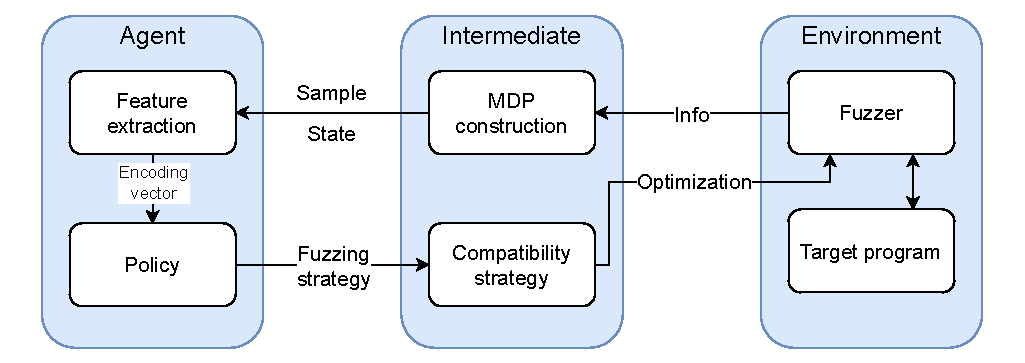
\includegraphics[width=0.9\textwidth]{fig/simplified_overview.pdf}}
	\caption{The overview of ALFruther.}
	\label{fig:overview}
\end{figure*}

Figure \ref{fig:overview} presents the overall structure of our approach, which implements a DRL-based fuzzing strategy optimization framework under real-world scenarios, as demonstrated in Section \ref{sec:background}. Our design comprises three primary components: MDP construction, agent processing, and compatibility strategies.

The MDP construction module continuously gathers real-time information in the fuzzing process, generating samples that capture state transitions. These samples are then processed by the agent processing module through a light-weight training workflow, along with optimizing the fuzzing strategy for each testcase. Finally, the compatibility strategies mediate the interaction between the fuzzer and the agent, reducing overhead and enhancing the overall efficiency of the fuzzing process.


\subsection{MDP Construction}\label{subsec:mdp_construction}

As detailed in Section \ref{subsubsec:markov_decision_process}, a Markov Decision Process (MDP) is formally specified by a four-tuple of elements: $(\mathcal{S}, \mathcal{A}, \mathcal{R}, T)$, where $\mathcal{S}$ denotes state, $\mathcal{A}$ action, $\mathcal{R}$ reward, and $T$ a terminal flag indicating whether an episode has ended. Since fuzzing usually entails consistent testing, we set $T=0$ by default, indicating that the fuzzing process would be non‑terminating until halted by external intervention or exceptions.

\subsubsection{State}\label{subsubsec:state}
% For each seed, execute a dry run and obtain bitmap.
A state contains the environment’s context at a given step. In our framework, each state originates from the following distinct components:
\begin{itemize}
	\item \textbf{Local Bitmap}: a binary bit map recording the hits of the code branches explored by the current testcase, reflecting the exploration status of local code coverage.
	\item \textbf{Global Bitmap}: a cumulative bitmap tracking all execution‑path visits during the fuzzing process, capturing global exploration history.
	\item \textbf{Sample Bytes}: the raw byte stream of the current testcase.
\end{itemize}
We encode each component for state construction as one channel of a three‑channel grayscale image. Specifically, we concatenate the local bitmap, global bitmap, and sample‑bytes representations along the channel dimension and then normalize the result to a fixed size of $256\times256$ via padding and clipping. The resolution offers a good trade‑off between data volume and processing efficiency, making it fit for the downstream model training.

\subsubsection{Action}
An action refers to the decision made by an agent to interact with its environment. In this study, we define an action as the fuzzing strategy guiding the mutation of a testcase. To quantize each fuzzer action, we collect the following features:
\begin{itemize} 
	\item \textbf{Seed weight}: the priority assigned to a seed, which influences the likelihood of its selection by the fuzzer.
	\item \textbf{Scheduling score}: an estimation value determining the computational resources allocated to each test case.
	\item \textbf{Mutation operator statistics}: historical records of mutation operations applied to a test case, including the frequency of choosing each mutation operator and the total number of mutation operations until discovering a new, valuable testcase.
\end{itemize}
To construct actions, we transform discrete operations into continuous strategies. Specifically, we normalize the distribution of each feature. The seed weight and scheduling score are normalized by the maximum value within the set of testcases:
\begin{align}
	\begin{split}
		\mathcal{A}_{\textit{sched}} &= \frac{\textit{score}}{\textit{score}_{\textit{max}}} \\
		\mathcal{A}_{\textit{weight}} &= \frac{\textit{weight}}{\textit{weight}_{\textit{max}}}
	\end{split}
\end{align}
Similarly, the mutation statistics are normalized to represent the probability of selecting each mutation operator:
\begin{equation}
	\mathcal{A}_{\textit{mut}, i} = \frac{count_{\textit{mut}, i}}{\sum_{j \in \textit{mut}} count_{\textit{mut}, j}}
\end{equation}
Finally, the action is constructed by concatenating the three normalized strategies.

\subsubsection{Reward}\label{subsubsec:reward}
Reward refers to a quantized metric to evaluate the profit that an agent obtains by policing based on a specific state of the explored environment. Considering the target of CGF is to maximize the code coverage, we define the reward function as the new paths discovered during a state transition locally and globally, which could be computed as: 
\begin{align}
	\begin{split}
		\textit{gain}_{l} &= \sum_{i=0}^{\textit{size}_{\textit{bitmap}} - 1} \max(0, \textit{bitmap}[i] - \textit{bitmap}_{\textit{parent}}[i]) \\
		\textit{gain}_{g} &= \sum_{i=0}^{\textit{size}_{\textit{bitmap}} - 1} \max(0, \textit{bitmap}[i] - \textit{bitmap}_{\textit{global}}[i])
	\end{split}
\end{align}
where $\textit{bitmap}_{\textit{parent}}$ refers to the bitmap of the parent testcase (namely $\mathcal{S}_{t-1}$).

In addition, it is significant to consider the energy (computation resources) cost assigned to each seed. Ignoring this aspect could lead the agent to allocate maximum energy to every seed, resulting in inefficiencies during fuzzing. Consequently, the reward is computed by incorporating both the scheduling score and the integration of the local and global coverage gains, using an $\epsilon$-greedy strategy:
\begin{equation}
	\mathcal{R} = (1 - \mathcal{A}_{\textit{sched}}) \cdot \left(\epsilon \cdot \textit{gain}_{l} + (1 - \epsilon) \cdot \textit{gain}_{g}\right)
	\label{eq:reward}
\end{equation}
where $\epsilon$ is a hyperparameter that ensures the balance between enhancing local exploration capability and maximizing global coverage.

\subsection{Agent}
\begin{figure}[t!]
	\centerline{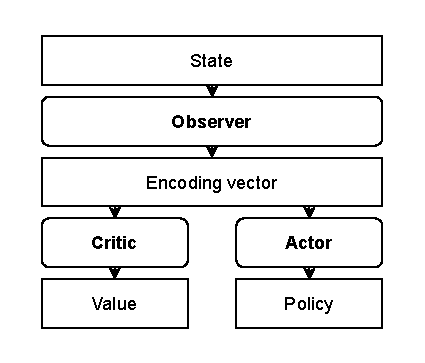
\includegraphics[width=0.5\textwidth]{fig/agent_structure2.pdf}}
	\caption{Agent Structure}
	\label{fig:agent_structure}
\end{figure}
An agent in DRL is a model to learn from environments and predict an optimal policy to maximize the reward. In our study, a lightweight agent is employed to learn the samples collected in Section \ref{subsec:sample_construction}, then predict the optimal fuzzing strategy for the testcases.

\subsubsection{Agent Architecture}
The agent structure follows the design of the actor–critic framework \cite{bartoNeuronlikeAdaptiveElements1983}. As illustrated in Figure \ref{fig:agent_structure}, the agent comprises three components:
\begin{itemize}
	\item \textbf{Observer}: implemented via a pretrained ResNet‑18 model \cite{heDeepResidualLearning2016}, this module extracts a compact feature vector from the high‑dimensional state images generated in Section \ref{subsubsec:state}, thereby reducing the computational cost of downstream training.
	\item \textbf{Critic}: a multi‑layer perceptron (MLP) that takes the feature and the normalized action vector as inputs, and produces an estimated value of the expected cumulative reward to optimize the agent.
	\item \textbf{Actor}: another three‑layer MLP that handles the feature vector and predicts the optimal fuzzing strategies to guide fuzzer mutation for performance improvement.
\end{itemize}

\subsubsection{Agent Training and Policing}

During the process, we implement the Prioritized Experience Replay (PER) \cite{schaulPrioritizedExperienceReplay2016} algorithm for sample replaying and the Soft Actor Critic (SAC) \cite{haarnojaSoftActorcriticOffpolicy2018} algorithm for the model training. PER algorithm could prioritize the samples with higher estimated errors, so that the model could converge faster, improving the efficiency of model training. At the same time, SAC is an offline RL training algorithm that learned experiences from the single-step state transition and predicts policies considering both maximum expected reward and explorability measured by entropy. Such a balance between exploration and exploitation could be adaptive with the nature of asynchronous exploration of fuzzing.

\begin{algorithm}[t!]
	\SetAlgoLined
	\DontPrintSemicolon
	\SetKwInOut{Input}{\texttt{\color{blue}Input}}
	\SetKwInOut{Output}{\texttt{\color{blue}Output}}
	% 设置关键字字体 参考文档10.8节
	%	\SetKwSty{texttt}
	
	%--------------------------------
	% 设置关键字 return 的颜色与加粗
	%	\SetKw{Return}
	%	{\textbf{\color{blue}return}}   % {return}
	%--------------------------------
	
	%--------------------------------
	% 设置关键字 break 的颜色与加粗
	\SetKw{Break}
	{\textbf{\color{blue}break}}
	%--------------------------------
	
	%--------------------------------
	% 设置关键字 and 的颜色与加粗
	\SetKw{And}
	{\textbf{\color{blue}and}}
	%--------------------------------
	
	%--------------------------------
	% 设置关键字 foreach 的颜色与加粗
	\SetKwFor{ForEach}
	{\textbf{\color{blue}foreach}}
	{\textbf{\color{blue}do}}
	{\textbf{\color{blue}end}}
	%--------------------------------
	
	%--------------------------------
	% 设置关键字 while 的颜色与加粗
	\SetKwFor{While}
	{\textbf{\color{blue}while}}    % {while}
	{\textbf{\color{blue}do}}       % {do}
	{\textbf{\color{blue}end}}
	%--------------------------------
	
	%--------------------------------
	% 设置关键字 if-else 的颜色与加粗
	\SetKwIF{If}{ElseIf}{Else}
	{\textbf{\color{blue}if}}       %{if}
	{\textbf{\color{blue}then}}     %{then}
	{\textbf{\color{blue}elif}}     %{elif}
	{\textbf{\color{blue}else}}     %{else}
	{\textbf{\color{blue}end}}
	%--------------------------------
	
	%--------------------------------
	% 设置关键字 function 的颜色与加粗
	%	\SetKwProg{Func}
	%	{\textbf{\color{blue}{function}}}
	%	{:}{}
	%--------------------------------	
	
	\KwIn{ Fuzzer to be optimized $Fuzzer$, training step $step_{train}$, decision step $step_{decision}$}
	%	\KwOut{bbb}
	\SetKwFunction{FuncScanDir}{\textbf{ScanDir}}
	\SetKwFunction{FuncNewSample}{\textbf{NewSample}}
	\SetKwFunction{FuncPolicy}{\textbf{Policy}}
	\SetKwFunction{FuncProcess}{\textbf{Process}}
	\SetKwFunction{FuncWrite}{\textbf{Write}}
	\SetKwProg{Fn}{Function}{:}{\KwRet}
	
	$\textit{SampleDir}$: sample directory\;
	$\textit{StateDir}$ state directory\;
	$\textit{PolicyDir}$ strategy directory\;
	$\textit{PER}$: PER sample buffer\;
	$\textit{size}$: batch size for each training\;
	$M$: model\;
	\BlankLine
	
	\Fn{\FuncProcess{$\textit{PER}$, $M$}}{
		%		\tcc{$dir$ is the directory storing samples, $M_{train}$ is training model, $M_{decicion}$ is decision model}
		%		initialize sample buffer $buf$\;
		\While{running}{
			%			$S\leftarrow$ \FuncGetNewSample{$dir$}
			$\textit{flag}$ = \textup{False}\;
			$\textit{List}_{\textit{sample}} \leftarrow$ \FuncScanDir{$\textit{SampleDir}$}\;
			\tcc{if $S$ is not empty, new samples exist, add to the buffer.}
			\If{$S$ = \FuncNewSample{$\textit{List}_{\textit{sample}}$			}}
			{
				$\textit{flag}$ = \textup{True}\;
				\ForEach{$s\in S$}{
					$\textit{PER}$.\textbf{add}($s$)\;
				}
			}
			
			\If{$\textit{flag}$}{
				$\textit{Batch}$ = $\textit{PER}$.\textbf{sample}($\textit{size}$)\;
				$\textit{errors}$ = $M$.\textbf{update}($\textit{Batch}$)\;\label{algline:model_update}
				$\textit{PER}$.\textbf{update}(\textit{errors})\;
				\tcc{after training, make policy for testcases.}
				$\textit{List}_\textit{state} \leftarrow$ \FuncScanDir{$\textit{StateDir}$}\;
				$\textit{List}_\textit{strategy} \leftarrow$ \FuncPolicy($M$, $\textit{List}_\textit{state}$)\;\label{algline:model_policy}
				\tcc{write strategy to disk for asynchronous reading from fuzzer.}
				\FuncWrite($\textit{List}_\textit{state}$, $\textit{PolicyDir}$)\;
				
			}
		}
	}
	
	\BlankLine
	
	\caption{Agent Process}\label{alg:agent_workflow}
\end{algorithm}


The agent workflow is illustrated in Algorithm \ref{alg:agent_workflow}. Note that the agent training in line \textbf{\ref{algline:model_update}} of the algorithm consists of observer, critic, and actor updates.
\begin{itemize}
	\item \textbf{observer and critic update}: The observer and critic network are trained to minimize the temporal difference errors between the expected and actual reward, updating the model to approximate the exploration environments. The loss function to update the critic could be presented as follows:
	\begin{equation}
		\mathcal{L}_{critic} = \| Q(\mathcal{S}_{t}, \mathcal{A}_t) - \hat{Q} \|^2
	\end{equation}
	where $\hat{Q}$ is the value expectation of the next state, which could be computed using the Bellman equation as:
	\begin{align}
		\begin{split}
			\hat{Q} = \mathcal{R}_t + \gamma \cdot Q_{\tau}(\mathcal{S}_{t+1}, \mathcal{A}_{t+1}) \\
			- \alpha \cdot \log \pi(\mathcal{A}_{t} | \mathcal{S}_{t})
		\end{split}
	\end{align}
	
	$Q_\tau$ refers to the expected value from another soft-update network, with the same architecture as the critic, whose role is to stabilize the model update. $\gamma$ and $\alpha$ are hyper-parameters, $\log \pi(\mathcal{A}_{t} | \mathcal{S}_{t})$ denotes the information entropy of the strategy $\mathcal{A}_t$ given the state $\mathcal{S}_t$, which could guarantee the model to explore more unknown states. Additionally, $\mathcal{A}_{t+1}$ refers to the predicted policy (fuzzing strategy) from the actor based on the next state.
	
	\item \textbf{Actor update}: The objective of the actor is to maximize the expected reward, which could be converted to minimize the negative of the estimated value. Additionally, the actor model should consider explorability by maximizing the entropy of an action. Therefore, the actor network is optimized using:
	\begin{equation}
		\mathcal{L}_{actor} = - \left( Q(\mathcal{S}_{t}, \mathcal{A}_t) - \alpha \cdot \log \pi(\mathcal{A}_{t} | \mathcal{S}_{t}) \right)
	\end{equation}
\end{itemize}

Besides, line \textbf{\ref{algline:model_policy}} refers to the optimal policy prediction of the agent for the testcases. At essence, the agent takes the state of a testcase and outputs a mean value ($\mu$) and a standard deviation ($\sigma$) to define a Gaussian distribution of the possible actions. The optimized strategy is then sampled from the distribution:

\begin{align} 
	\begin{split}
		\mu, \sigma &= \textit{Policy}(S) \\ 
		\mathcal{F} &\sim \mathcal{N}(\mu, \sigma^2) 
	\end{split}
\end{align}

Such an approach ensures the policy is optimized while incorporating the randomness for exploration. By sampling from the Gaussian distribution, the agent effectively balances the trade-off between exploration (seeking new strategy) and exploitation (leveraging optimized strategy to obtain high rewards), similar to the insights in prior studies \cite{jauernigDARWINSurvivalFittest2023}.

\subsection{Compatibility Strategy}
As detailed in Section \ref{subsec:challenge}, we employ the following compatibility strategies to seamlessly integrate the DRL framework with the fuzzer while minimizing implementation overhead.

\subsubsection{Training}
In contrast to traditional DRL methods used in simulated environments, we implement training the agent and predicting strategies only when new samples are encountered, as outlined in Algorithm \ref{alg:agent_workflow}. This approach eliminates the need for redundant model training and sample processing, reducing computational overhead. Furthermore, common DRL methods typically utilize mini-batch training and asynchronous model updates to maintain performance and stability at each step. In contrast our approach processes only a single batch of samples and updates the model synchronously at each step. Since fuzzing involves high throughput and smooth, chronological evolution of fuzzing status, such a strategy would be better suited for the process. Consequently, the training strategies could effectively balance the trade-off between model training performance and fuzzing efficiency.
% only have new samples.
% one step one batch
% update every step
\subsubsection{Policing}
% sampling
Since fuzzing requires high throughput and potentially generates tremendous testcases, we implement a specific policing strategy inspired by mini-batching techniques. Specifically, the framework would update the fuzzing strategies for only a subset of testcases at each step, selected by random sampling, which prioritized the new testcases. Such an approach could guarantee the improvement of the fuzzing strategy while substantially reducing the overhead associated with policy prediction, mediating its influence on fuzzing performance.

\subsubsection{Integration}\label{subsubsec:integration}

A fundamental difference between DRL and fuzzing lies in the characteristics of their exploration processes. DRL requires initial exploration before policy optimization, whereas fuzzing performs exploration and optimization concurrently. As a result, if the integrated framework strictly follows the DRL approach, the DRL's influence on the fuzzing process will be minimal during the initial phase, and the timing of implementing optimization would be difficult to determine. On the other hand, if the fuzzing strategy fully adopts the strategy predicted by the agent before it is fully trained, the exploration process will be severely disrupted. In both scenarios, fuzzing performance will be compromised significantly.

To address the issue, we propose a warm-up scheduling strategy based on the cosine annealing algorithm. Specifically, during the initial phase of the fuzzing process, we introduce a scheduler that determines whether to employ the fuzzing strategy derived from the DRL policy with a certain probability. The probability is calculated as follows:

\begin{equation}
	P_{\textit{DRL}} = \frac{1}{2}\left(1 - \cos\left(\frac{\min(T_{\textit{cur}}, T_{\textit{max}})}{T_{\textit{max}}}\pi\right)\right)
	\label{eq:cosine_scheduling}
\end{equation}

As fuzzing progresses, the scheduling probability would gradually increase, eventually fully transitioning to DRL-based strategies upon reaching a predefined time threshold $T_{\textit{max}}$. Consequently, the scheduling approach could facilitate a smooth integration of DRL policies while allowing the DRL framework to learn sufficient exploration experience, improving overall performance.

\section{Implementation}
We have developed an ALFurther prototype consisting of approximately 900 C and Python code lines. Specifically, the implementation is divided into two main modules: the fuzzer module and the agent module.
\begin{itemize}
	\item \textbf{Fuzzer Module}: The module is implemented as an extension of AFL++ 4.21a. It is responsible for constructing the Markov Decision Process (MDP) and implementing DRL-based policies. For MDP construction, a collector gathers relevant information during the fuzzing process. The module also constructs samples with normalized states and actions for agent training. Additionally, suppose a test case does not discover any new testcases by the end of the current test period. In that case, the module saves the ending state as a negative sample, ensuring a sufficient volume of samples for training. Regarding policy implementation, the module retrieves the optimized strategy for the current test case from disk if available and replaces the original strategies with DRL-based policies during fuzzing.
	
	\item \textbf{Agent Module}: The module incorporates a sample buffer based on PER and a SAC-based agent model. The buffer's capacity is set to 100,000 to balance memory usage and performance. For the SAC module, the learning rate is set to 0.0003, and the batch size is configured to 32. Additionally, the hidden dimension of all MLP models is set to 256. The agent module begins operating after accumulating 256 samples, ensuring adequate initial exploration before the training.
\end{itemize}
The hyperparameters include an $\epsilon$ value of 0.1 in Equation \ref{eq:reward} and a maximum scheduling time, $T_{\textit{max}}$, of 2 hours in Equation \ref{eq:cosine_scheduling}, both of which are determined through controlled experiments. Additionally, a file control lock is employed in both the fuzzer and agent modules to minimize conflicts arising from file synchronization.

\begin{table*}[t!]
	\centering
	\caption{Compared fuzzers.}
	\begin{tabularx}{\textwidth}{p{5.2cm}M{3.3cm}L}
		\toprule
		\multicolumn{1}{c}{\textbf{Type}} & \multicolumn{1}{c}{\textbf{Fuzzer}} & \multicolumn{1}{c}{\textbf{Description}} \\
		\midrule
		\multicolumn{1}{l}{heuristic-based fuzzing optimization} & AFL++~\cite{fioraldiAFLCombiningIncremental2020} & baseline and implementation prototype \\
		\midrule
		\multicolumn{1}{l}{\multirow{2}[4]{*}{seed scheduling optimization}} & AFLfast~\cite{bohmeCoveragebasedGreyboxFuzzing2019} & seed scheduling based on Markov chain \\
		\cmidrule{2-3}          & EcoFuzz~\cite{yueEcoFuzzAdaptiveEnergysaving2020} & seed scheduling based on MDP and adverserial MAB \\
		\midrule
		\multicolumn{1}{l}{\multirow{2}[4]{*}{mutation strategy optimization}} & MOPT~\cite{lyuMOPTOptimizedMutation2019} & optimze mutation strategy based on swarm intelligence algorithm \\
		\cmidrule{2-3}          & DARWIN~\cite{jauernigDARWINSurvivalFittest2023} & optimize mutation strategy using perturbation and evolution algorithm \\
		\bottomrule
	\end{tabularx}%
	\label{tab:compared_fuzzer}%
\end{table*}%

\section{Evaluation}\label{sec:evaluation}
In this section, we evaluate the ALFurther to answer the following questions:
\begin{itemize}
	\item \textbf{RQ1}: Would ALFurther improve the code coverage of the CGF?
	\item \textbf{RQ2}: Would ALFurther improve the bug discovery of the CGF?
	\item \textbf{RQ3}: How does the DRL-based process impact the fuzzing overhead?
	\item \textbf{RQ4}: How does DRL-based optimization impact the reward of fuzzing?
\end{itemize}

\subsection{Experiment Settings}

\subsubsection{Compared Fuzzers}

The fuzzers compared in our study are summarized in Table \ref{tab:compared_fuzzer}. We selected these fuzzers based on their relevance to our research objectives and the feasibility of evaluation. Specifically, AFL++ serves as the prototype for our implementation. AFLfast and EcoFuzz are optimization-based fuzzers focusing on seed scheduling strategies, whereas MOPT and DARWIN are designed to optimize mutation scheduling strategies.

\subsubsection{Benchmarks}
We evaluated ALFurther on two public benchmarks: Unibench \cite{liUNIFUZZHolisticPragmatic2021} and MAGMA \cite{hazimehMagmaGroundtruthFuzzing2021}. Unibench contains 24 collected real-world programs containing bugs, which could be adopted for evaluating both coverage and bug discovery. MAGMA consists of real-world open source projects that delicately inject bugs and ground truths for the type and location of the bugs, providing a more comprehensive analysis of the bug discovery capability of fuzzers.

\begin{table}[t!]
	\centering
	\caption{Target programs from Unibench}
	\begin{tabularx}{\linewidth}
		{ 
			LLCp{2.2cm}
			%			>{\raggedright\arraybackslash}X
			%			>{\raggedright\arraybackslash}X 
			%			>{\raggedleft\arraybackslash}X 
			%			>{\raggedright\arraybackslash}X 
		}
	%	\begin{tabular}{llrl}
		\toprule
		\textbf{Targets} & \textbf{Projects} & \multicolumn{1}{l}{\textbf{Total edges}} & \textbf{Parameters} \\
		\midrule
		cflow & cflow-1.6 & 4620  & "@@" \\
		flvmeta & flvmeta-1.2.1 & 3711  & "@@" \\
		imginfo & jasper-2.0.12 & 12040 & "-f @@" \\
		infotocap & ncurses-6.1 & 6037  & "-o /dev/null @@" \\
		jhead & jhead-3.00 & 1107  & "@@" \\
		jq    & jq-1.5 & 5604  & "@@" \\
		mp3gain & mp3gain-1.5.2 & 1619  & "@@" \\
		mp42aac & Bento4-1.5.1 & 13592 & "@@" \\
		mujs  & mujs-1.0.2 & 13369 & "@@" \\
		objdump & binutils-2.28 & 42848 & "-S @@" \\
		pdftotext & xpdf-4.00 & 26720 & "@@ /dev/null" \\
		tcpdump & libpcap-1.8.1 & 25806 & "-e -vv -nr @@" \\
		tiffsplit & libtiff-3.9.7 & 5336  & "@@" \\
		\bottomrule
	\end{tabularx}%
	\label{tab:Unibench_program}%
\end{table}%

In our evaluation, we employed 12 targets from the Unibench suite, with their statistics summarized in Table~\ref{tab:Unibench_program}. Other targets were excluded due to various issues, including compilation errors (\textit{exiv}, \textit{wav2swf}, \textit{gdk}), testing failures (\textit{objdump}, \textit{ffmpeg}, \textit{nm-new}, \textit{sqlite3}, \textit{lame}), and obsolescence (\textit{uniq}, \textit{base64}, \textit{md5sum}, \textit{who} from the LAVA-M dataset~\cite{dolan-gavittLAVALargescaleAutomated2016}). For the MAGMA evaluation, \textit{json}, \textit{parser}, \textit{unserialize} from \textit{php} project due to failure testing, and \textit{pdf\_fuzzer}, \textit{pdfimages}, \textit{pdftoppm} were excluded due to a compilation incompatibility involving \textit{libbzip2} between \textit{poppler} and ALFurther. These excluded programs may be evaluated in future work once the underlying issues are resolved.

For evaluation, AFL++, AFLfast, EcoFuzz, and MOPT were evaluated on both the Unibench and MAGMA benchmarks. Additionally, Unibench included DARWIN in its evaluation as a supplementary.

\subsubsection{Evaluation Metrics}
We adopt the following metrics to evaluate the performance of the fuzzers:
\begin{itemize}
	\item \textbf{Edge Coverage}: Measures the number of unique edges exercised, reflecting the fuzzer's capability in coverage discovery.
	\item \textbf{Crash Count}: Measures the number of unique crashes discovered, reflecting the fuzzer's bug-finding capability.
	\item \textbf{Bug Exposure Time}: Measures the time required to reach or trigger a bug, specifically defined in MAGMA, to evaluate the efficiency of bug discovery.
\end{itemize}
Additionally, we employed several specific metrics in the ablation study to further investigate the features of ALFurther.

\subsubsection{Environment}
The experiments were conducted on a server with an Intel Xeon (R) Gold 6258R CPU, 256 GB of RAM, and two Nvidia RTX 4090 GPUs, running Debian 12. Each trial was executed within an isolated Docker container with an independent agent model to ensure fairness, thereby preventing interference across different runs.

\subsection{Coverage Exploration}\label{subsec:evaluation_coverage}


To answer \textbf{RQ1}, we evaluated the edge coverage achieved by each fuzzer across 12 available programs in the Unibench benchmark, conducting 10 independent runs of 24 hours each. All test cases were re-analyzed to ensure fairness using afl-cov on GCC-compiled binaries \cite{AFLplusplusAflcov2025}. During the experiments, all fuzzers were configured to skip the deterministic stage, following the recommendations of previous work \cite{metzmanFuzzBenchOpenFuzzer2021}. Statistical significance was assessed using the Mann-Whitney U test to compare the results.

The average edge coverage attained by each fuzzer is presented in Table~\ref{tab:edge_coverage}. A p-value $<$ 0.05 indicates that the differences observed are statistically significant. The results show that ALFurther achieved the highest edge coverage in 6 out of 12 programs and outperformed the prototype AFL++ in 7 of 12 cases. Notably, ALFurther demonstrated a maximum improvement of 10\% over AFL++ in \textit{infotocap}, with the largest observed decrease being less than 0.1\% in \textit{pdftotext}. These findings confirm the effectiveness and robustness of DRL-based fuzzing optimization for coverage exploration.

One thing to be admitted is that our method has not significantly improved performance based on the prototype AFL++. However, it should also be noted that the results gaps among all fuzzers are not huge. The findings indicate that the current optimization-based approach may confront the bottleneck in improvement due to the slow development of heuristic-based fuzzing techniques, and the situation may only be improved by more innovative progress in coverage-guided fuzzing. Nonetheless, our method could still outperform in half of all targets, which validates the guarantee of the optimality of the DRL method. Furthermore, since the method has no limits on the target optimization, the framework could be transferred to other implementations once new methods appear.

The mean edge coverage gained by the fuzzers over time is depicted in Figure \ref{fig:unibench_edge_cov}. Interestingly, ALFurther always performs behind AFL++ for the first few hours. However, it commonly overwhelms the baseline as the fuzzing continues. Such a finding reveals the mechanism of DRL: at the initial stage, DRL focuses on the exploration of the environment, thus may not perform so ideally; nonetheless, the method would gradually improve during the fuzzing process, contributed by the continuous learning, and finally have better performance. Furthermore, it could be seen that ALFurther may maintain a higher tendency in coverage improvement at the end stage of the evaluation, as presented in Figure \ref{fig:coverage-infotocap}, \ref{fig:coverage-pdftotext},\ref{fig:coverage-tiffsplit}. Such a phenomenon implies that ALFurther may have better effectiveness in longer fuzzing tests with continuous learning and exploration from the environment, which may fit better in practical fuzzing evaluation scenarios (which may continue testing for weeks, months, or even years), which could be evaluated in the derivative work.

Answer to \textbf{RQ1}: ALFurther could achieve better coverage performance in 6 of 12 evaluated programs among the compared fuzzers, validating that the method could improve the effectiveness of fuzzing in coverage exploration with robustness.

\begin{table*}[t!]
	\centering
	\caption{The mean edge coverage of the fuzzers on 12 real programs from Unibench. p-value $<$ 0.05 indicates that the experiments are statistically significant.}
	\begin{tabular}{lccccccccccr}
		\toprule
		\multicolumn{1}{c}{\multirow{2}[4]{*}{\textbf{program}}} & \textbf{ALFuther} & \multicolumn{2}{c}{\textbf{AFL++}} & \multicolumn{2}{c}{\textbf{AFLfast}} & \multicolumn{2}{c}{\textbf{DARWIN}} & \multicolumn{2}{c}{\textbf{EcoFuzz}} & \multicolumn{2}{c}{\textbf{MOPT}} \\
		\cmidrule{2-12}          & \textbf{coverage} & \textbf{coverage} & \textbf{p-value} & \textbf{coverage} & \textbf{p-value} & \textbf{coverage} & \textbf{p-value} & \textbf{coverage} & \textbf{p-value} & \textbf{coverage} & \multicolumn{1}{c}{\textbf{p-value}} \\
		\midrule
		cflow & \multicolumn{1}{r}{1227.1} & \multicolumn{1}{r}{1228.3 } & \multicolumn{1}{r}{0.3515 } & \multicolumn{1}{r}{1233.0 } & \multicolumn{1}{r}{0.0002 } & \multicolumn{1}{r}{\textbf{1233.4 }} & \multicolumn{1}{r}{0.0002 } & \multicolumn{1}{r}{1231.7 } & \multicolumn{1}{r}{0.0006 } & \multicolumn{1}{r}{1232.5 } & 0.0002  \\
		flvmeta & \multicolumn{1}{r}{\textbf{321.6}} & \multicolumn{1}{r}{321.0 } & \multicolumn{1}{r}{0.4704 } & \multicolumn{1}{r}{314.4 } & \multicolumn{1}{r}{0.0001 } & \multicolumn{1}{r}{315.7 } & \multicolumn{1}{r}{0.0001 } & \multicolumn{1}{r}{314.5 } & \multicolumn{1}{r}{0.0001 } & \multicolumn{1}{r}{315.3 } & 0.0001  \\
		imginfo & \multicolumn{1}{r}{\textbf{2342.5}} & \multicolumn{1}{r}{2240.0 } & \multicolumn{1}{r}{0.0058 } & \multicolumn{1}{r}{2166.5 } & \multicolumn{1}{r}{0.0002 } & \multicolumn{1}{r}{2195.3 } & \multicolumn{1}{r}{0.0002 } & \multicolumn{1}{r}{2224.7 } & \multicolumn{1}{r}{0.0002 } & \multicolumn{1}{r}{2235.4 } & 0.0002  \\
		infotocap & \multicolumn{1}{r}{\textbf{1698.9}} & \multicolumn{1}{r}{1533.6 } & \multicolumn{1}{r}{0.0638 } & \multicolumn{1}{r}{1567.4 } & \multicolumn{1}{r}{0.5708 } & \multicolumn{1}{r}{1674.7 } & \multicolumn{1}{r}{0.6776 } & \multicolumn{1}{r}{1294.7 } & \multicolumn{1}{r}{0.0003 } & \multicolumn{1}{r}{1580.7 } & 0.4727  \\
		jhead & \multicolumn{1}{r}{\textbf{214.0}} & \multicolumn{1}{r}{\textbf{214.0 }} & \multicolumn{1}{r}{1.0000 } & \multicolumn{1}{r}{213.9 } & \multicolumn{1}{r}{0.3681 } & \multicolumn{1}{r}{213.6 } & \multicolumn{1}{r}{0.0336 } & \multicolumn{1}{r}{\textbf{214.0 }} & \multicolumn{1}{r}{1.0000 } & \multicolumn{1}{r}{213.9 } & 0.3681  \\
		jq    & \multicolumn{1}{r}{1893} & \multicolumn{1}{r}{\textbf{1893.7 }} & \multicolumn{1}{r}{0.8489 } & \multicolumn{1}{r}{1881.8 } & \multicolumn{1}{r}{0.0005 } & \multicolumn{1}{r}{1890.9 } & \multicolumn{1}{r}{0.1954 } & \multicolumn{1}{r}{1883.8 } & \multicolumn{1}{r}{0.0010 } & \multicolumn{1}{r}{1885.9 } & 0.0688  \\
		mp3gain & \multicolumn{1}{r}{965.4} & \multicolumn{1}{r}{969.2 } & \multicolumn{1}{r}{0.4725 } & \multicolumn{1}{r}{\textbf{999.0 }} & \multicolumn{1}{r}{0.0036 } & \multicolumn{1}{r}{998.4 } & \multicolumn{1}{r}{0.0101 } & \multicolumn{1}{r}{944.3 } & \multicolumn{1}{r}{0.0691 } & \multicolumn{1}{r}{996.3 } & 0.0090  \\
		mp42aac & \multicolumn{1}{r}{1448.7} & \multicolumn{1}{r}{1392.0 } & \multicolumn{1}{r}{0.0311 } & \multicolumn{1}{r}{1390.7 } & \multicolumn{1}{r}{0.0036 } & \multicolumn{1}{r}{\textbf{1486.1 }} & \multicolumn{1}{r}{0.0638 } & \multicolumn{1}{r}{1305.9 } & \multicolumn{1}{r}{0.0025 } & \multicolumn{1}{r}{1423.4 } & 0.3254  \\
		mujs  & \multicolumn{1}{r}{\textbf{2764.2}} & \multicolumn{1}{r}{2719.5 } & \multicolumn{1}{r}{0.0072 } & \multicolumn{1}{r}{2664.2 } & \multicolumn{1}{r}{0.0002 } & \multicolumn{1}{r}{2669.5 } & \multicolumn{1}{r}{0.0002 } & \multicolumn{1}{r}{2603.2 } & \multicolumn{1}{r}{0.0002 } & \multicolumn{1}{r}{2719.2 } & 0.0045  \\
		pdftotext & \multicolumn{1}{r}{7386.3} & \multicolumn{1}{r}{7398.5 } & \multicolumn{1}{r}{0.8501 } & \multicolumn{1}{r}{7722.3 } & \multicolumn{1}{r}{0.0002 } & \multicolumn{1}{r}{7664.5 } & \multicolumn{1}{r}{0.0091 } & \multicolumn{1}{r}{6731.8 } & \multicolumn{1}{r}{0.0002 } & \multicolumn{1}{r}{\textbf{7726.3 }} & 0.0008  \\
		tcpdump & \multicolumn{1}{r}{\textbf{335.9}} & \multicolumn{1}{r}{333.1 } & \multicolumn{1}{r}{0.0151 } & \multicolumn{1}{r}{329.2 } & \multicolumn{1}{r}{0.0015 } & \multicolumn{1}{r}{331.1 } & \multicolumn{1}{r}{0.0049 } & \multicolumn{1}{r}{329.7 } & \multicolumn{1}{r}{0.0057 } & \multicolumn{1}{r}{331.6 } & 0.0015  \\
		tiffsplit & \multicolumn{1}{r}{1526.4} & \multicolumn{1}{r}{1461.1 } & \multicolumn{1}{r}{0.0757 } & \multicolumn{1}{r}{1528.7 } & \multicolumn{1}{r}{0.4727 } & \multicolumn{1}{r}{\textbf{1575.2 }} & \multicolumn{1}{r}{0.0693 } & \multicolumn{1}{r}{1405.9 } & \multicolumn{1}{r}{0.0036 } & \multicolumn{1}{r}{1547.7 } & 1.0000  \\
		\midrule
		\textbf{Max num} & 6     & 2     &       & 1     &       & 3     &       & 1     &       & 1     &  \\
		\bottomrule
	\end{tabular}%
	\label{tab:edge_coverage}%
\end{table*}%

\begin{figure*}[t!]
	%	\centerline{
		\subfloat[\centering\normalsize cflow\label{fig:coverage-cflow}]{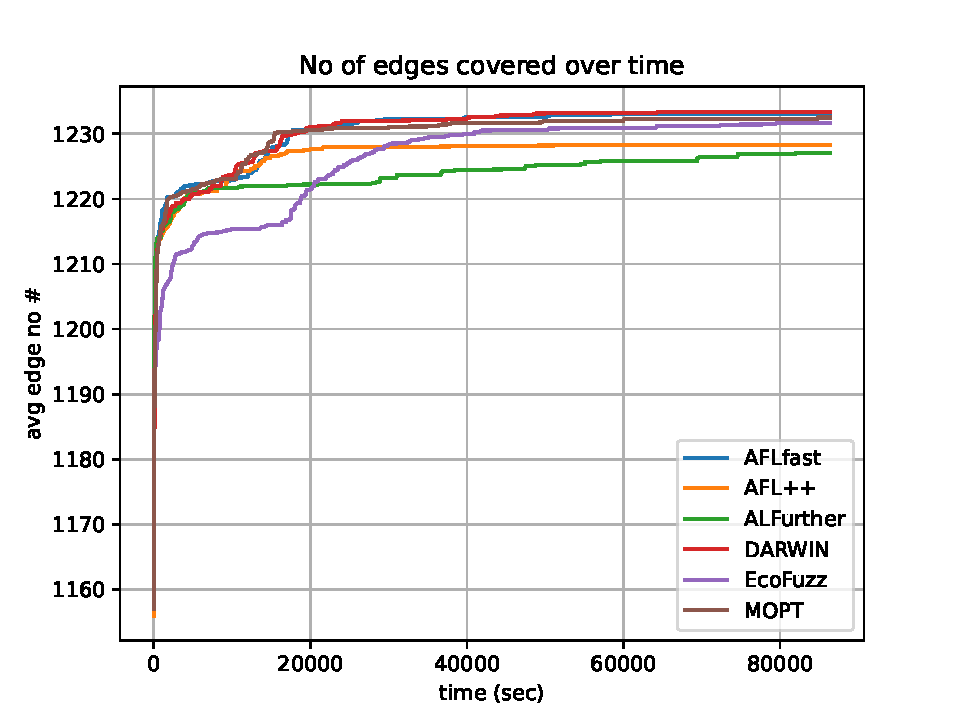
\includegraphics[width=0.25\textwidth]{results/coverage/cflow_edge_cov.pdf}}
		\subfloat[\centering\normalsize flvmeta\label{fig:coverage-flvmeta}]{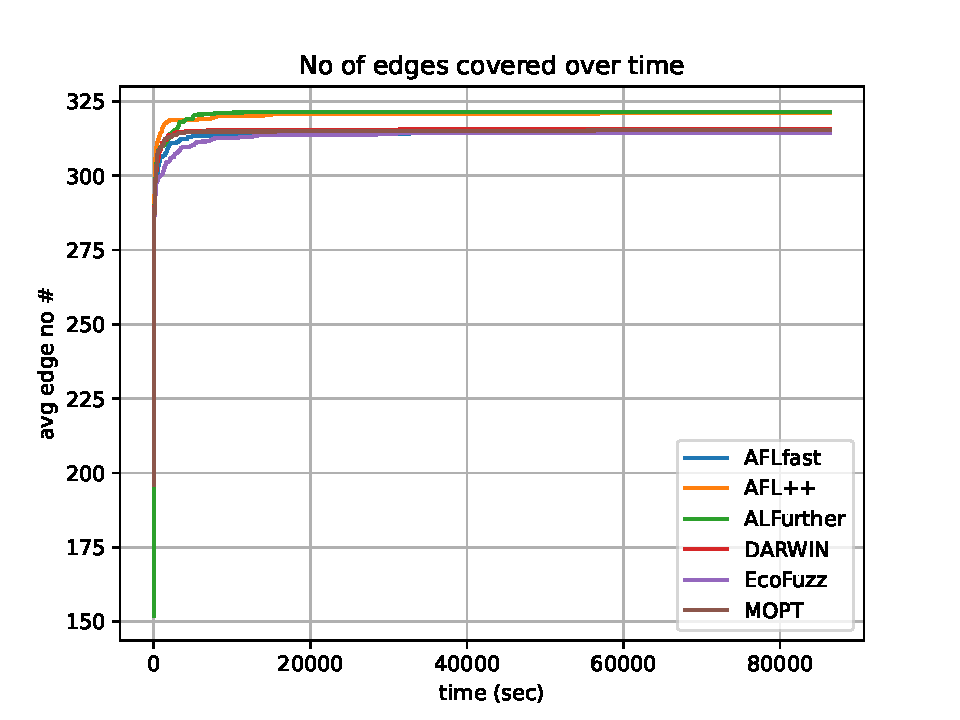
\includegraphics[width=0.25\textwidth]{results/coverage/flvmeta_edge_cov.pdf}}
		\subfloat[\centering\normalsize imginfo\label{fig:coverage-imginfo}]{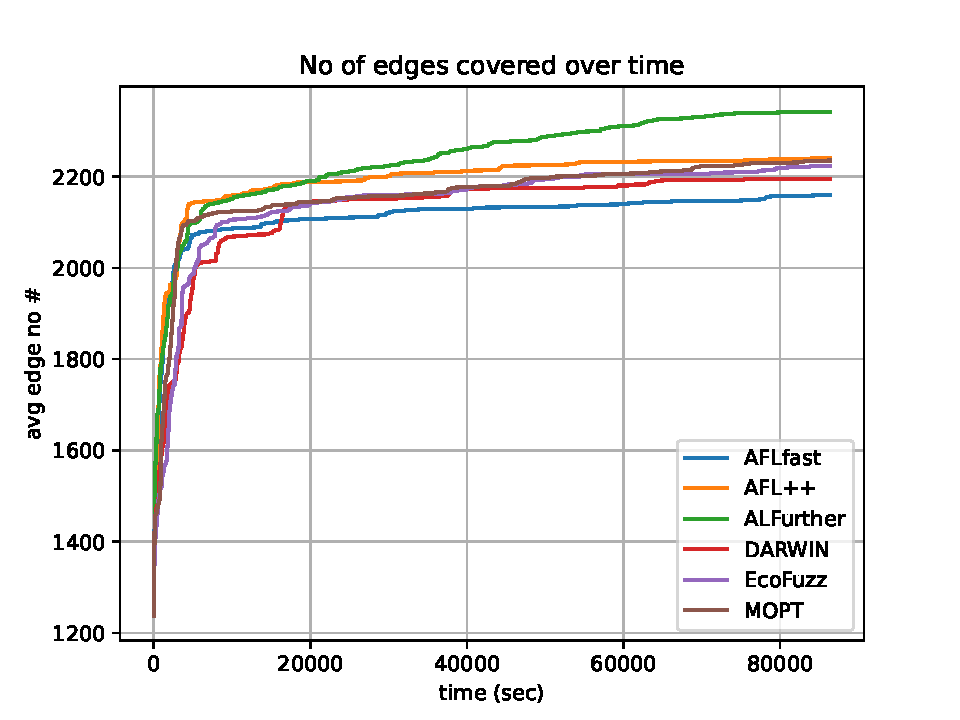
\includegraphics[width=0.25\textwidth]{results/coverage/imginfo_edge_cov.pdf}}
		\subfloat[\centering\normalsize infotocap\label{fig:coverage-infotocap}]{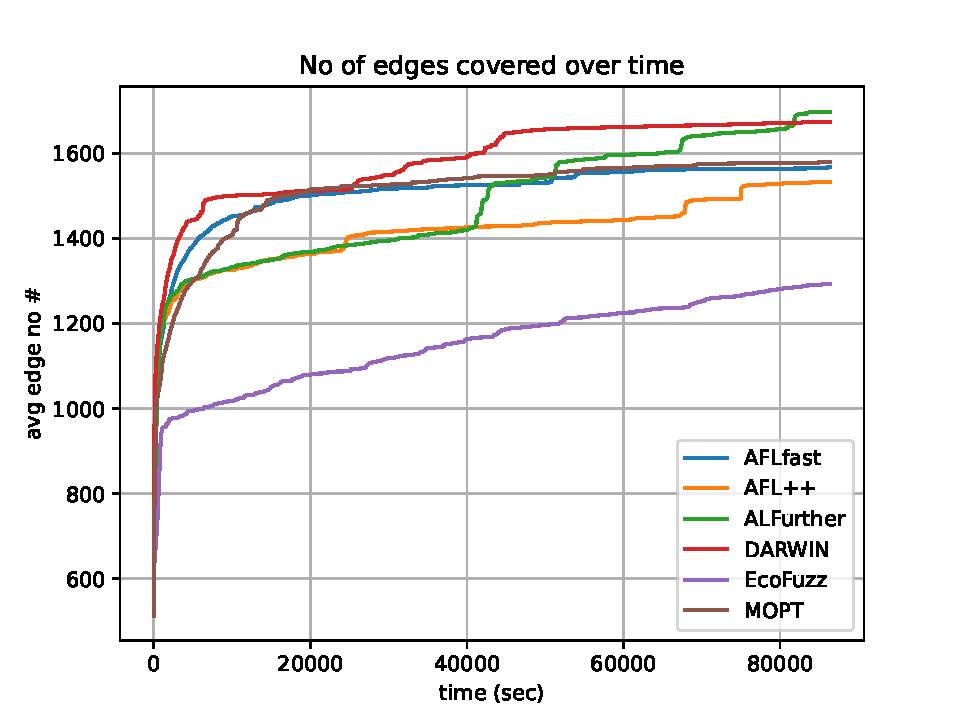
\includegraphics[width=0.25\textwidth]{results/coverage/infotocap_edge_cov.pdf}}
		\\
		\subfloat[\centering\normalsize jhead\label{fig:coverage-jhead}]{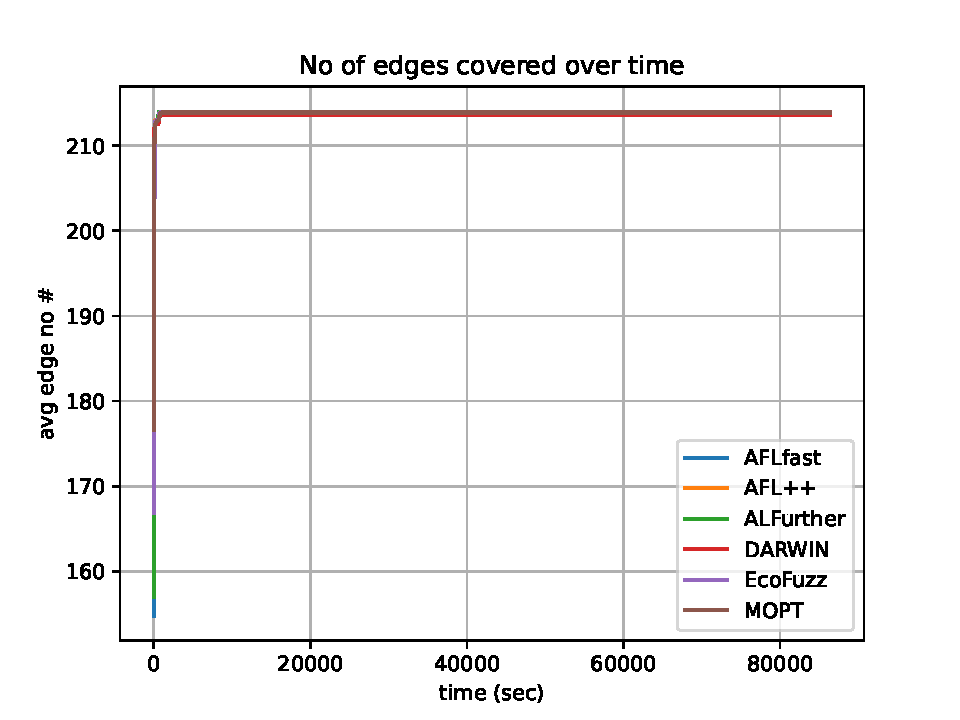
\includegraphics[width=0.25\textwidth]{results/coverage/jhead_edge_cov.pdf}}
		\subfloat[\centering\normalsize jq\label{fig:coverage-jq}]{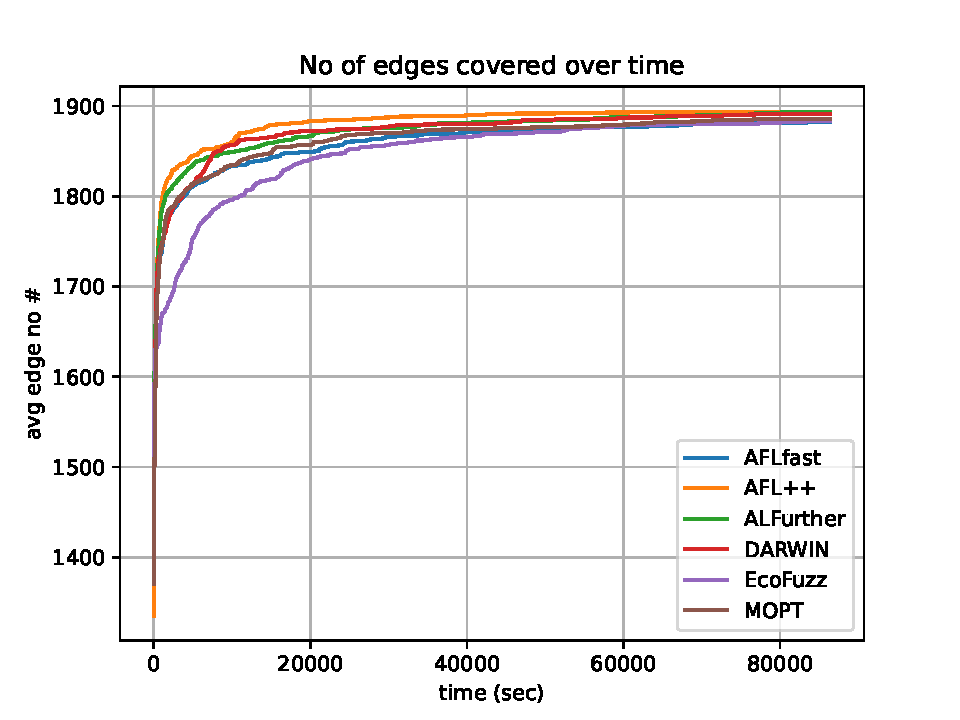
\includegraphics[width=0.25\textwidth]{results/coverage/jq_edge_cov.pdf}}
		\subfloat[\centering\normalsize mp3gain\label{fig:coverage-mp3gain}]{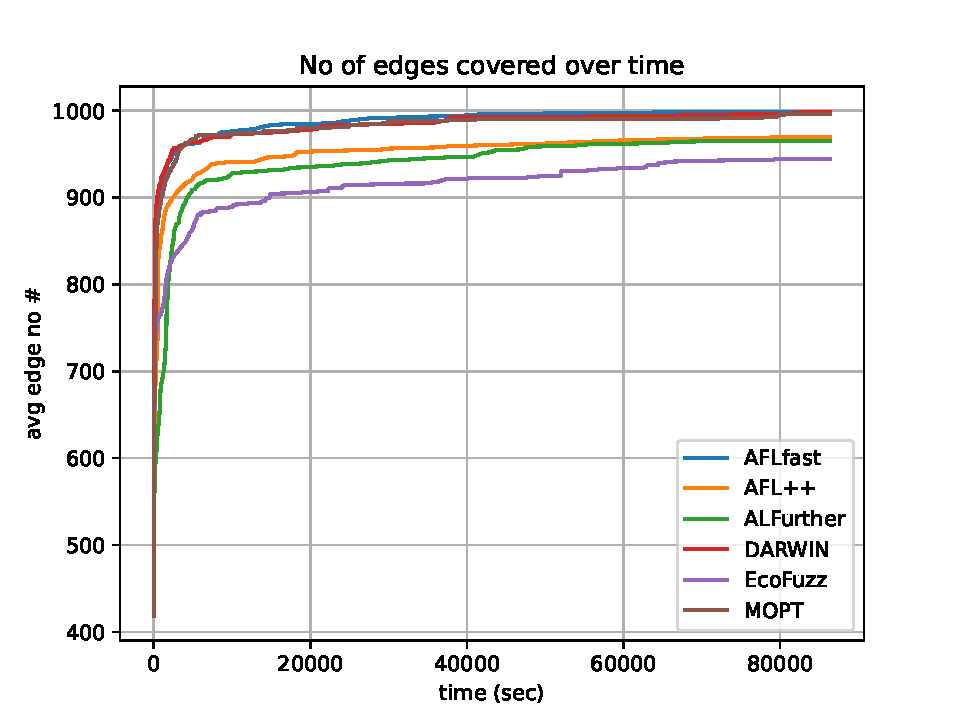
\includegraphics[width=0.25\textwidth]{results/coverage/mp3gain_edge_cov.pdf}}
		\subfloat[\centering\normalsize mp42aac\label{fig:coverage-mp42aac}]{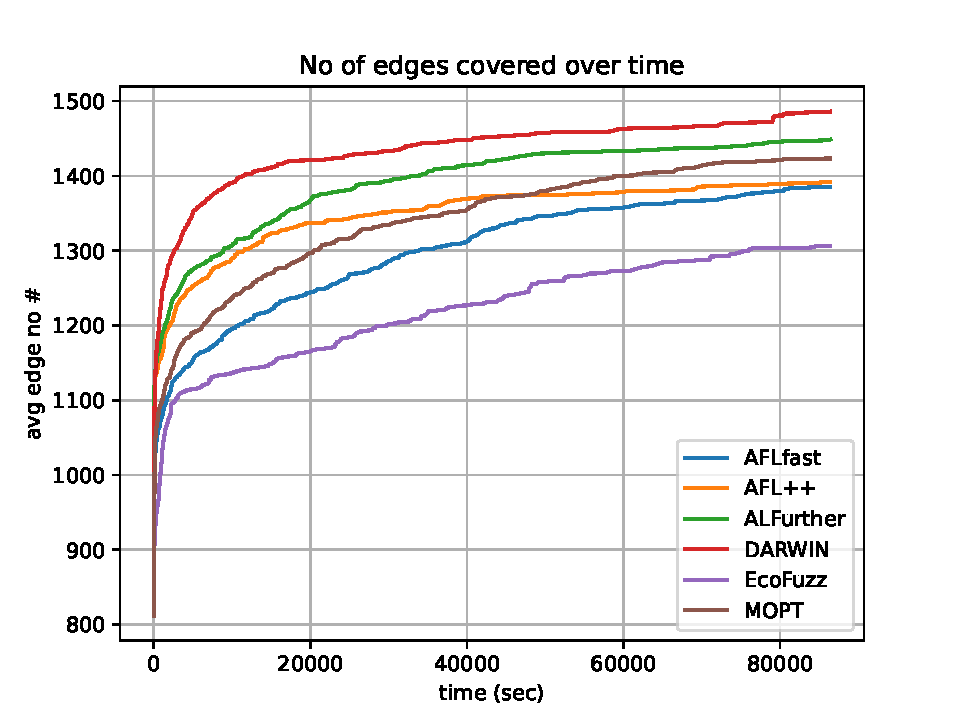
\includegraphics[width=0.25\textwidth]{results/coverage/mp42aac_edge_cov.pdf}}
		\\
		\subfloat[\centering\normalsize mujs\label{fig:coverage-mujs}]{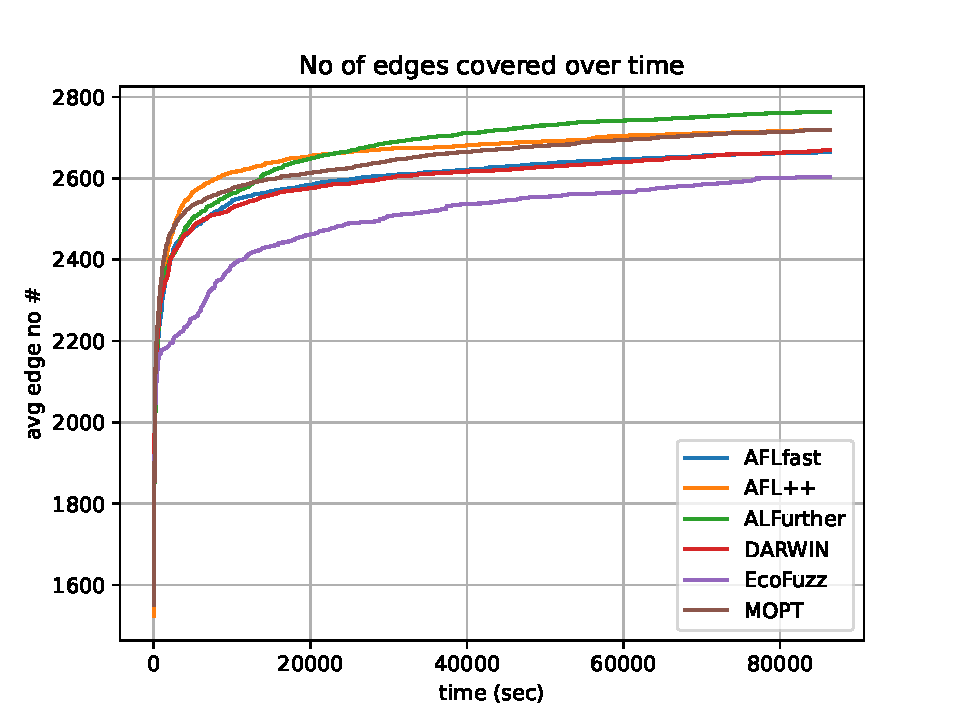
\includegraphics[width=0.25\textwidth]{results/coverage/mujs_edge_cov.pdf}}
		\subfloat[\centering\normalsize pdftotext\label{fig:coverage-pdftotext}]{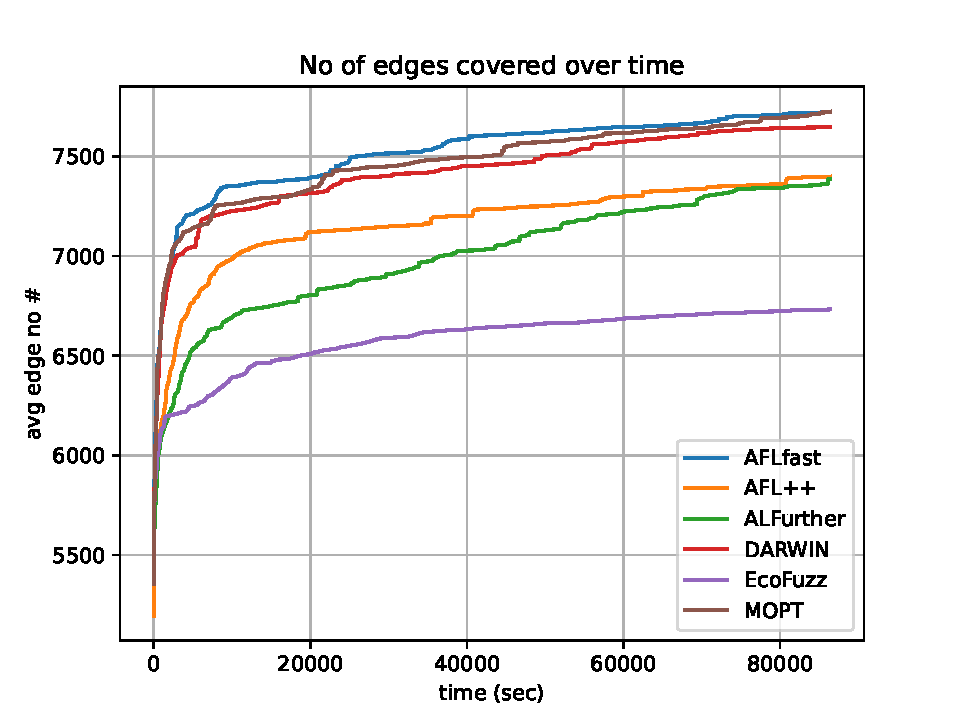
\includegraphics[width=0.25\textwidth]{results/coverage/pdftotext_edge_cov.pdf}}
		\subfloat[\centering\normalsize tcpdump\label{fig:coverage-tcpdump}]{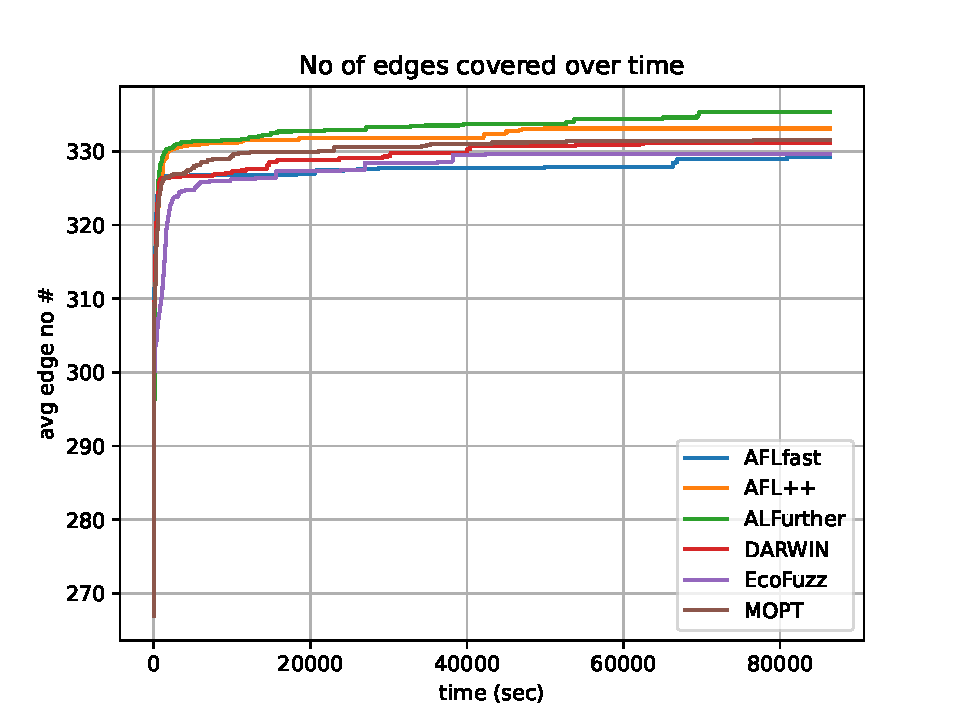
\includegraphics[width=0.25\textwidth]{results/coverage/tcpdump_edge_cov.pdf}}
		\subfloat[\centering\normalsize tiffsplit\label{fig:coverage-tiffsplit}]{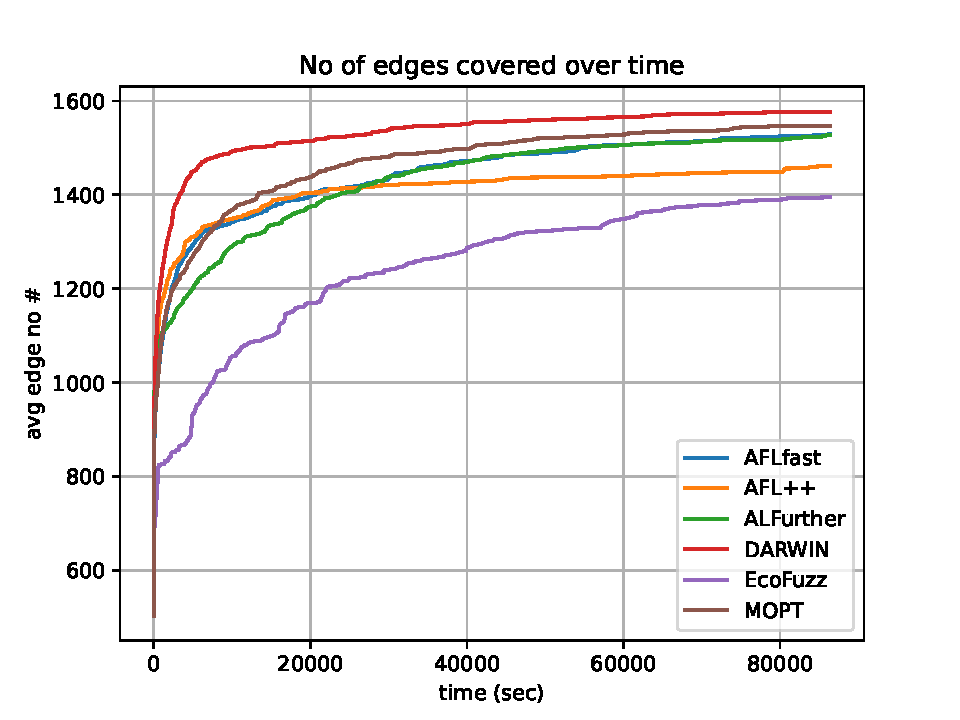
\includegraphics[width=0.25\textwidth]{results/coverage/tiffsplit_edge_cov.pdf}}
		%	}
	\caption{The average number of coverages discovered by ALFruther and other fuzzers over 24 hours and 10 runs.}
	\label{fig:unibench_edge_cov}
\end{figure*}
\subsection{Bug Discovery}

We evaluate ALFurther using both the Unibench and MAGMA benchmarks. Notably, Unibench assesses fuzzer effectiveness based on the number of unique crashes discovered, whereas MAGMA provides a more comprehensive evaluation of bug discovery performance.


\subsubsection{Unibench Crash Analysis}
\begin{figure*}[t!]
	%	\centerline{
		\subfloat[\centering\normalsize cflow\label{fig:crash-cflow}]{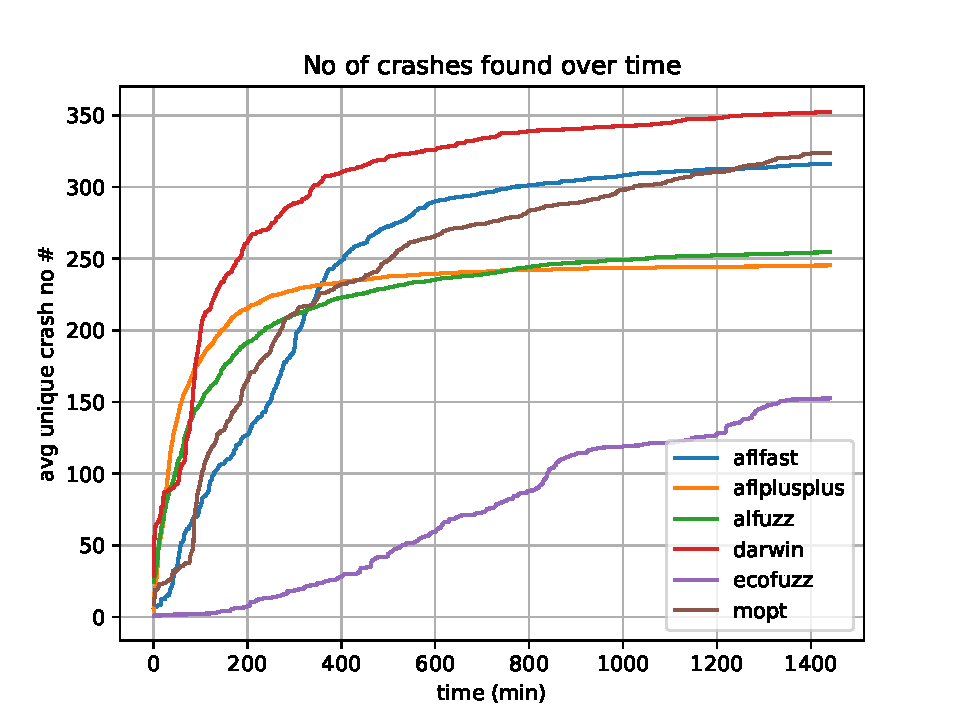
\includegraphics[width=0.33\textwidth]{results/crash/cflow_crash.pdf}}
		\subfloat[\centering\normalsize flvmeta\label{fig:crash-flvmeta}]{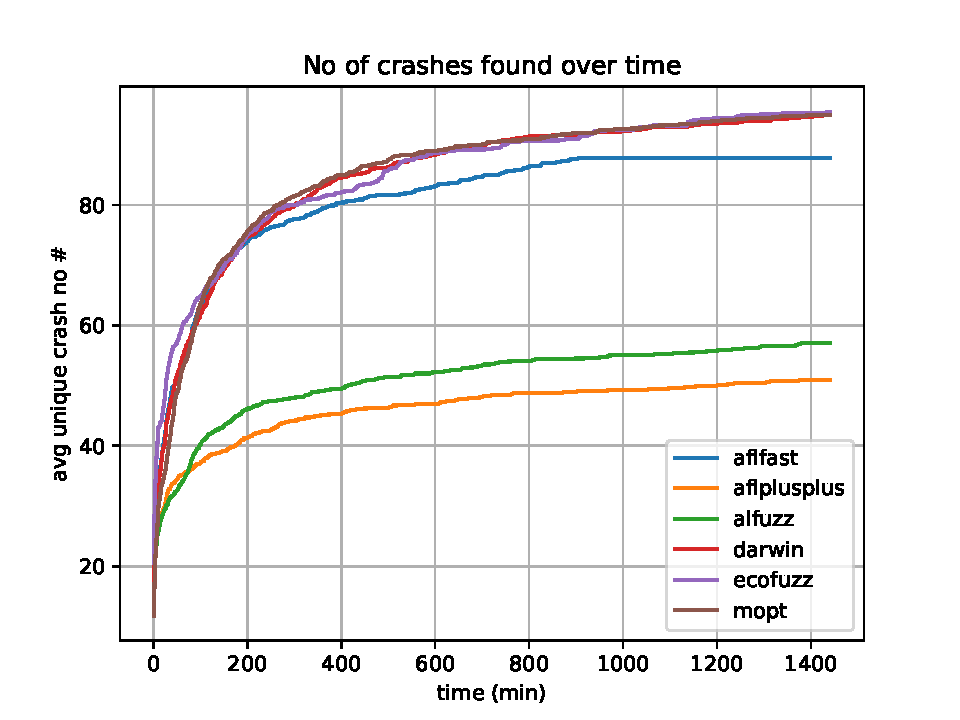
\includegraphics[width=0.33\textwidth]{results/crash/flvmeta_crash.pdf}}
		\subfloat[\centering\normalsize mp3gain\label{fig:crash-mp3gain}]{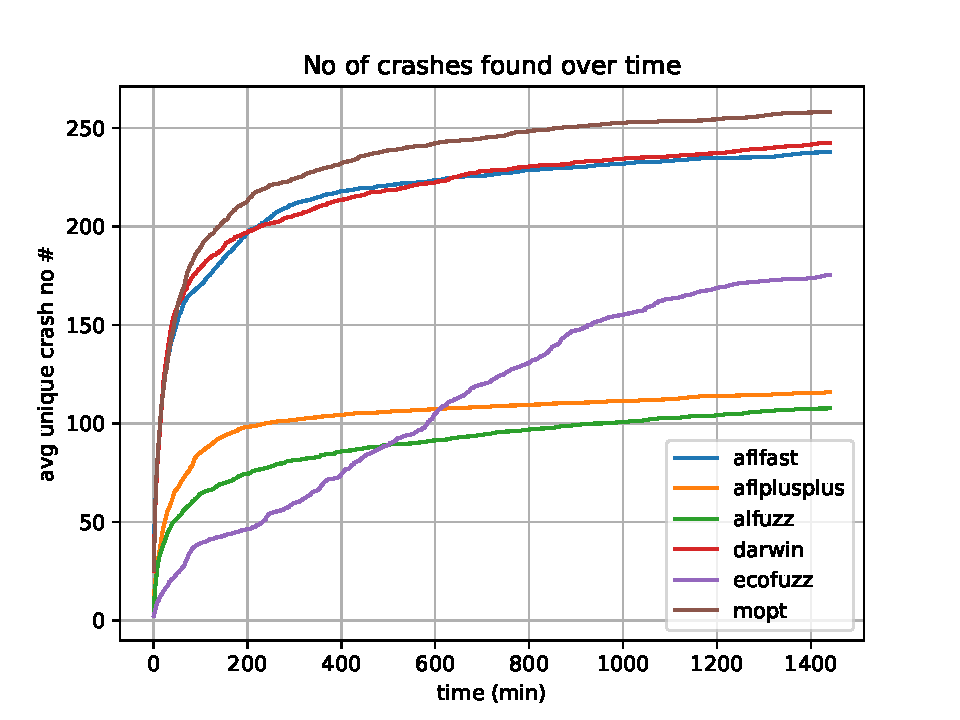
\includegraphics[width=0.33\textwidth]{results/crash/mp3gain_crash.pdf}}
		\\
		\subfloat[\centering\normalsize mp42aac\label{fig:crash-mp42aac}]{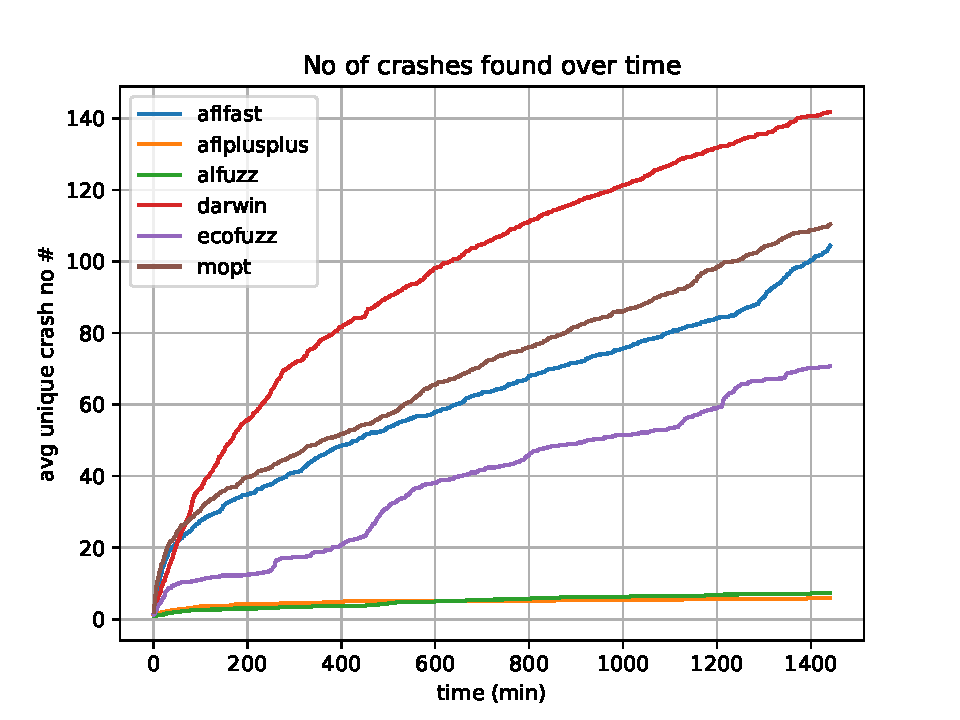
\includegraphics[width=0.33\textwidth]{results/crash/mp42aac_crash.pdf}}
		\subfloat[\centering\normalsize pdftotext\label{fig:crash-pdftotext}]{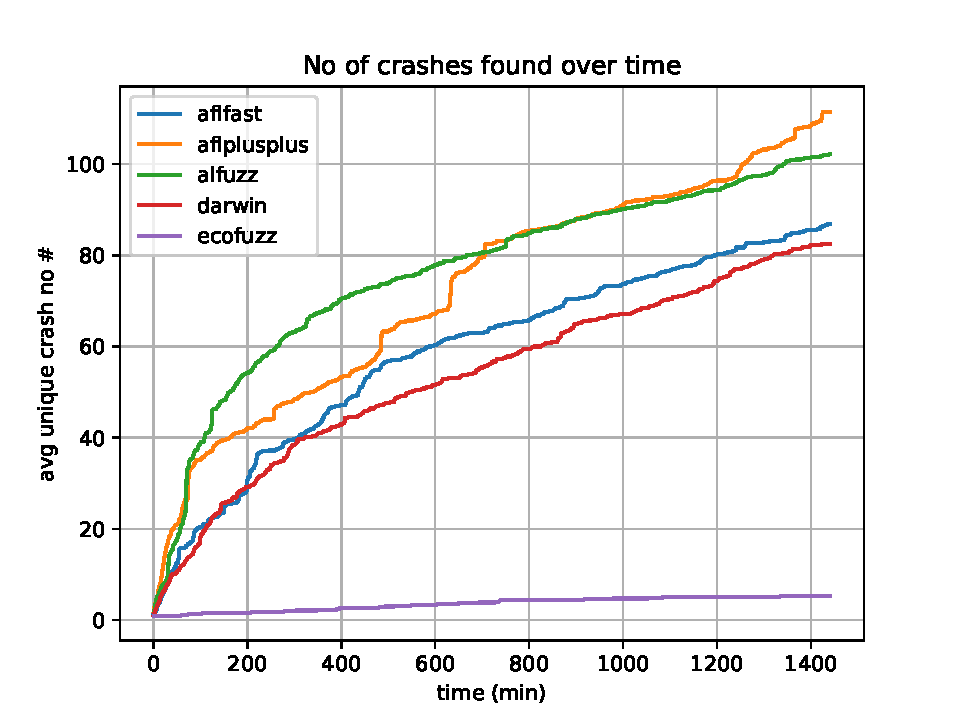
\includegraphics[width=0.33\textwidth]{results/crash/pdftotext_crash.pdf}}
		\subfloat[\centering\normalsize tiffsplit\label{fig:crash-tiffsplit}]{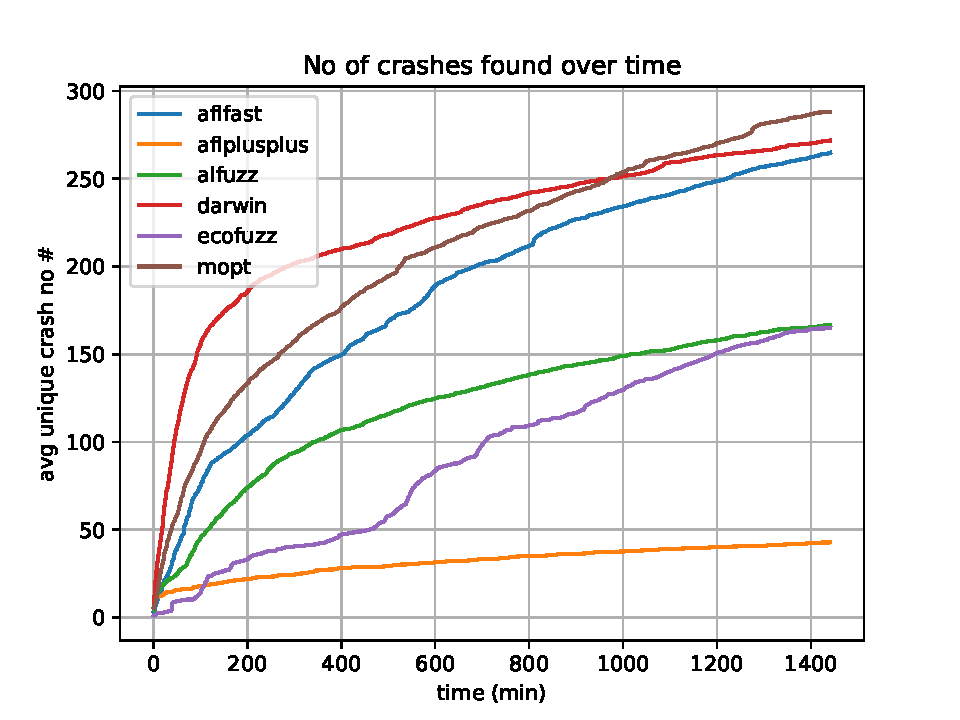
\includegraphics[width=0.33\textwidth]{results/crash/tiffsplit_crash.pdf}}
		%	}
	\caption{The average number of crashes discovered by ALFruther and other fuzzers over 24 hours and 10 runs.}
	\label{fig:unibench_crash}
\end{figure*}

The average number of unique crashes discovered by each fuzzer on Unibench is summarized in Table \ref{tab:unique_crash}. The program \textit{jq} is omitted from the results, as no crashes were identified by any of the fuzzers. To ensure accuracy, all crashes were re-evaluated using AFLTriage \cite{QuicAFLTriage2025} on binaries instrumented with AddressSanitizer (ASAN) \cite{serebryanyAddressSanitizerFastAddress2012}. As shown in the table, ALFurther discovered 13.5 more unique crashes than AFL++ in total. However, both ALFurther and AFL++ were outperformed by AFLfast, DARWIN, and MOPT, suggesting there is still room for improvement.

For a deeper understanding, Figure \ref{fig:unibench_crash} illustrates the number of unique crashes identified by each fuzzer over time. Due to limited data, only representative results are presented. The results indicate that AFLfast, DARWIN, and MOPT were able to discover substantially more crashes within the first 200 minutes of fuzzing compared to ALFurther and AFL++, except in the case of \textit{pdftotext}. One possible explanation for this difference is the use of different instrumentation methods (\textit{afl-cc} for AFL-based fuzzers vs. \textit{afl-clang} for AFL++ and ALFurther), which may have a significant impact on crash detection and warrants further investigation.
Additionally, ALFurther outperformed AFL++ in 4 out of 6 programs. The exceptions, \textit{mp3gain} and \textit{pdftotext}, are consistent with the edge coverage results shown in Table \ref{tab:edge_coverage}. These findings suggest that the improvement in ALFurther’s bug discovery capability is primarily attributable to its enhanced coverage exploration.



\begin{table}[t!]
	\centering
	\caption{The mean unique crashes of fuzzers on 12 real programs from Unibench}
	\resizebox{\linewidth}{!}{
		\begin{tabular}{lrrrrrr}
			\toprule
			\multicolumn{1}{c}{\textbf{Program}} & \multicolumn{1}{c}{\textbf{ALFurther}} & \multicolumn{1}{c}{\textbf{AFL++}} & \multicolumn{1}{c}{\textbf{AFLfast}} & \multicolumn{1}{c}{\textbf{DARWIN}} & \multicolumn{1}{c}{\textbf{EcoFuzz}} & \multicolumn{1}{c}{\textbf{MOPT}} \\
			\midrule
			cflow & 43.2  & 32.8  & 55.9  & \textbf{75.5} & 22.3  & 57.0  \\
			flvmeta & 5.1   & 4.3   & 7.9   & \textbf{9.1} & 6.3   & 8.3  \\
			imginfo & \textbf{0.9} & 0.1   & 0.0   & 0.1   & 0.4   & 0.4  \\
			infotocap & 2.1   & 1.1   & 3.1   & \textbf{3.6} & 0.7   & 3.0  \\
			jhead & 1.6   & 2.7   & 1.5   & \textbf{4.9} & 1.2   & 2.1  \\
			mp3gain & 8.1   & 7.5   & \textbf{10.8} & 10.4  & 8.6   & 10.0  \\
			mp42aac & 0.0   & 0.0   & 0.0   & 0.0   & \textbf{0.3} & 0.0  \\
			mujs  & 0.9   & 0.8   & 0.5   & \textbf{3.2} & 0.2   & 0.7  \\
			pdftotext & 10.2  & 13.1  & 15.0  & 16.9  & 2.1   & \textbf{17.9} \\
			tcpdump & 0.1   & 0.0   & 0.0   & \textbf{0.3} & 0.2   & 0.0  \\
			tiffsplit & 10.0  & 6.3   & 12.1  & 11.5  & 9.6   & \textbf{13.1} \\
			\midrule
			\textbf{Sum} & 82.2  & 68.7  & 106.8  & 135.5  & 51.9  & 112.5  \\
			\bottomrule
		\end{tabular}%
	}
	\label{tab:unique_crash}%
\end{table}%



\subsubsection{MAGMA Bug Analysis}\label{subsubsec:magma_analysis}

\begin{table*}[t!]
	\centering
	\caption{The average numbers of bugs reached (\textbf{R}) and triggered (\textbf{T}) by the fuzzers on the MAGMA benchmark, evaluated over 10 independent runs each lasting 24 hours.}
	\begin{tabularx}{\textwidth}{LCCcCCcCCcCC}
		\toprule
		\multicolumn{1}{c}{\multirow{2}[4]{*}{\textbf{Program}}} & \multicolumn{2}{c}{\textbf{ALFurther}} &       & \multicolumn{2}{c}{\textbf{AFL++}} &       & \multicolumn{2}{c}{\textbf{AFLFast}} &       & \multicolumn{2}{c}{\textbf{MOPT}} \\
		\cmidrule{2-12}          & \textbf{R} & \textbf{T} &       & \textbf{R} & \textbf{T} &       & \textbf{R} & \textbf{T} &       & \textbf{R} & \textbf{T} \\
		\midrule
		asn1  & 4     & 2     &       & 4     & 1.9   &       & 4     & 1     &       & 4     & 1.2 \\
		asn1parse & 1     & 0     &       & 1     & 0     &       & 1     & 0     &       & 1     & 0 \\
		bignum & 1     & 0     &       & 1     & 0     &       & 1     & 0     &       & 1     & 0 \\
		client & 7     & 1     &       & 7     & 1     &       & 7     & 1     &       & 7     & 1 \\
		exif  & 5     & 2.5   &       & 5     & 2.2   &       & 5     & 3     &       & 5     & 3 \\
		libpng & 6     & 3     &       & 6     & 2.3   &       & 6     & 1     &       & 6     & 1.7 \\
		libxml2 & 8     & 2.8   &       & 8.1   & 4     &       & 8     & 1.3   &       & 8     & 2.9 \\
		server & 6     & 1     &       & 6     & 1     &       & 6     & 2     &       & 6     & 1.8 \\
		sndfile & 8     & 7     &       & 8     & 7     &       & 8     & 2     &       & 8     & 7 \\
		sqlite3 & 11.4  & 3.1   &       & 11.1  & 3.1   &       & 8.5   & 1.3   &       & 9.8   & 2.6 \\
		tiff\_read & 5.7   & 3.1   &       & 5.8   & 3     &       & 5.4   & 2.5   &       & 6.7   & 3.8 \\
		tiffcp & 8.5   & 6.1   &       & 7     & 4.8   &       & 5.7   & 3.4   &       & 6.6   & 4.4 \\
		x509  & 5     & 0     &       & 5     & 0     &       & 5     & 0.6   &       & 5     & 0.7 \\
		xmllint & 7     & 1.9   &       & 7     & 2     &       & 7     & 2     &       & 7.1   & 2.5 \\
		\midrule
		\textbf{Sum} & 83.6  & 33.5  &       & 82    & 32.3  &       & 77.6  & 21.1  &       & 81.2  & 32.6 \\
		\bottomrule
	\end{tabularx}%
	\label{tab:magma_count}%
\end{table*}%

Table \ref{tab:magma_count} presents the average number of bugs reached (\textbf{R}) and triggered (\textbf{T}) by each fuzzer on the MAGMA benchmark, measured over ten 24-hour runs. As AFLfast cannot collect Lua-specific statistics, results for this target are omitted from the AFLfast column; the complete dataset without AFLfast is provided in Appendix \ref{appdx:magma_lua}. According to the table, ALFurther achieves the highest counts for both bugs reached and triggered among all evaluated fuzzers. Notably, compared to AFL++, ALFurther discovers more bugs on the majority of targets, demonstrating that, although primarily optimized for coverage, ALFurther also enhances bug-finding effectiveness, consistent with observations in prior work \cite{bohmeFuzzingExponentialCost2020}.

A direct comparison between ALFurther and AFL++ shows that ALFurther reaches more bugs in two programs (\textit{sqlite3} and \textit{tiffcp}) and triggers more bugs in five (\textit{asn1}, \textit{exif}, \textit{libpng}, \textit{tiff\_read}, and \textit{tiffcp}). This trend suggests that ALFurther’s advantage may stem more from superior mutation selection and exploitation, leading to deeper exploration of bug-rich regions than purely exploratory improvements. This hypothesis warrants further investigation.

To provide a finer-grained perspective, Table \ref{tab:bug_time} reports the average time required by each fuzzer to reach and trigger specific bugs, yielding several insights. While ALFurther generally required more time to reach bugs than AFL++, achieving faster reachability in only 19 out of 60 programs, it is important to note that most delays (28 programs) involved reaching times within a single minute, with an average delay of only 6.87 seconds. This minor overhead is likely attributable to the initial setup and configuration of the RL modules. If this bias of approximately six seconds is discounted, ALFurther would surpass AFL++ in reaching bugs for 30 out of 60 programs, making its performance more competitive.

In contrast, ALFurther demonstrated substantial gains in bug-triggering efficiency, triggering bugs faster than AFL++ in 19 out of 31 cases, with an average improvement of $2.26\times$. This notable speedup underscores the effectiveness of our proposed method in expediting bug triggering. Furthermore, ALFurther exhibited robust bug-triggering performance in large and complex software projects, such as \textit{php}, \textit{sqlite}, \textit{libpng}, and \textit{libxml}, indicating its efficacy in challenging, real-world scenarios. The maximum observed improvements were substantial, with ALFurther triggering bugs up to $14.1\times$ (\textit{SND005}) and $15.3\times$ (\textit{PHP009}) faster than AFL++, highlighting the considerable potential of DRL-based fuzzing optimizations.

Nevertheless, MOPT achieved the best overall performance in terms of bug discovery times, consistent with previous studies \cite{hazimehMagmaGroundtruthFuzzing2021,metzmanFuzzBenchOpenFuzzer2021}. ALFurther did not outperform MOPT, likely due to fundamental differences in their optimization objectives: while MOPT is explicitly designed to identify “interesting” test cases—including those that trigger bugs \cite{lyuMOPTOptimizedMutation2019}—ALFurther is optimized primarily for coverage maximization, as discussed in Section \ref{subsec:evaluation_coverage}. Consequently, improvements in bug discovery can be seen as a beneficial side effect of enhanced coverage. To further improve ALFurther’s effectiveness in bug discovery, future work could incorporate feedback mechanisms related to crash discovery efficiency, which may offer a promising avenue for advancing bug-triggering performance.

\textbf{Answer to RQ2}: ALFurther enhances bug discovery effectiveness relative to its prototype AFL++, achieving the highest MAGMA benchmark bug counts. In addition, it significantly improves bug-triggering efficiency compared to the baseline. However, ALFurther does not achieve the best results across all fuzzers regarding crash discovery and bug discovery times, possibly due to the current reward function design. Addressing this limitation could be an important direction for future research.






\begin{table}[t!]
	\centering
	\caption{The average times required by the fuzzers to reach (\textbf{R}) and trigger (\textbf{T}) bugs on the MAGMA benchmark, computed over 10 independent runs with a time budget of 24 hours each.}
	\resizebox{\linewidth}{!}{
		\begin{tabular}{lrrrrrrrr}
			\toprule
			\multicolumn{1}{c}{\multirow{2}[4]{*}{\textbf{Bug ID}}} & \multicolumn{2}{c}{\textbf{ALFurther}} & \multicolumn{2}{c}{\textbf{AFL++}} & \multicolumn{2}{c}{\textbf{AFLfast}} & \multicolumn{2}{c}{\textbf{MOPT}} \\
			\cmidrule{2-9}          & \multicolumn{1}{c}{\textbf{R}} & \multicolumn{1}{c}{\textbf{T}} & \multicolumn{1}{c}{\textbf{R}} & \multicolumn{1}{c}{\textbf{T}} & \multicolumn{1}{c}{\textbf{ R}} & \multicolumn{1}{c}{\textbf{T}} & \multicolumn{1}{c}{\textbf{R}} & \multicolumn{1}{c}{\textbf{T}} \\
			\midrule
			PHP002 & 28.5  & \multicolumn{1}{l}{-} & 10.0  & \multicolumn{1}{l}{-} & 15.0  & \multicolumn{1}{l}{-} & 15.0  & \multicolumn{1}{l}{-} \\
			PHP003 & 29.0  & \multicolumn{1}{l}{-} & 15.0  & \multicolumn{1}{l}{-} & 15.0  & \multicolumn{1}{l}{-} & 15.0  & \multicolumn{1}{l}{-} \\
			PHP004 & 26.0  & 2987.0  & 15.0  & 14940.0  & 15.0  & 1369.0  & 15.0  & 3400.5  \\
			PHP009 & 26.0  & 2063.0  & 15.0  & 31750.0  & 15.0  & 19939.0  & 15.0  & 5212.5  \\
			PHP011 & 18.0  & 380.5  & 15.0  & 2306.0  & 10.0  & 11756.5  & 10.0  & 81.0  \\
			\midrule
			PNG001 & 20.0  & \multicolumn{1}{l}{-} & 15.0  & \multicolumn{1}{l}{-} & 15.0  & \multicolumn{1}{l}{-} & 15.0  & \multicolumn{1}{l}{-} \\
			PNG003 & 15.0  & 32.5  & 15.0  & 52.0  & 10.0  & 15.0  & 10.0  & 21.5  \\
			PNG004 & 25.0  & \multicolumn{1}{l}{-} & 16.5  & \multicolumn{1}{l}{-} & 15.0  & \multicolumn{1}{l}{-} & 24.0  & \multicolumn{1}{l}{-} \\
			PNG005 & 20.0  & \multicolumn{1}{l}{-} & 15.0  & \multicolumn{1}{l}{-} & 15.0  & \multicolumn{1}{l}{-} & 15.0  & \multicolumn{1}{l}{-} \\
			PNG006 & 20.0  & 132.5  & 10.0  & 335.5  & 15.0  & \multicolumn{1}{l}{-} & 15.0  & \multicolumn{1}{l}{-} \\
			PNG007 & 20.0  & 31479.0  & 15.0  & 40273.3  & 15.0  & \multicolumn{1}{l}{-} & 15.0  & 32660.7  \\
			\midrule
			SND001 & 25.0  & 914.5  & 20.5  & 1496.5  & 452.0  & \multicolumn{1}{l}{-} & 15.0  & 709.0  \\
			SND005 & 19.0  & 11112.5  & 268.5  & 7514.0  & 10.0  & 5713.5  & 10.0  & 134.5  \\
			SND006 & 25.0  & 1728.0  & 19.0  & 4954.0  & 452.0  & \multicolumn{1}{l}{-} & 15.0  & 861.5  \\
			SND007 & 25.0  & 4409.0  & 19.0  & 3541.0  & 452.0  & \multicolumn{1}{l}{-} & 15.0  & 867.5  \\
			SND016 & 24.0  & \multicolumn{1}{l}{-} & 10.0  & \multicolumn{1}{l}{-} & 452.0  & \multicolumn{1}{l}{-} & 15.0  & \multicolumn{1}{l}{-} \\
			SND017 & 2699.0  & 2895.5  & 1360.0  & 1439.0  & 452.0  & 467.0  & 75.5  & 121.5  \\
			SND020 & 4951.0  & 9551.5  & 2346.0  & 2580.0  & 2501.5  & \multicolumn{1}{l}{-} & 113.0  & 1222.5  \\
			SND024 & 25.0  & 1726.0  & 15.5  & 2739.0  & 452.0  & \multicolumn{1}{l}{-} & 15.0  & 856.0  \\
			\midrule
			SQL002 & 68.0  & 3796.0  & 286.5  & 20463.5  & 4555.0  & 50100.6  & 59.5  & 4968.0  \\
			SQL003 & 51757.5  & \multicolumn{1}{l}{-} & 26320.0  & \multicolumn{1}{l}{-} & \multicolumn{1}{l}{-} & \multicolumn{1}{l}{-} & \multicolumn{1}{l}{-} & \multicolumn{1}{l}{-} \\
			SQL006 & 34387.5  & \multicolumn{1}{l}{-} & \multicolumn{1}{l}{-} & \multicolumn{1}{l}{-} & \multicolumn{1}{l}{-} & \multicolumn{1}{l}{-} & 64830.0  & \multicolumn{1}{l}{-} \\
			SQL007 & 59.5  & \multicolumn{1}{l}{-} & 287.0  & \multicolumn{1}{l}{-} & 4680.5  & \multicolumn{1}{l}{-} & 51.5  & \multicolumn{1}{l}{-} \\
			SQL009 & 1897.0  & \multicolumn{1}{l}{-} & 2829.5  & \multicolumn{1}{l}{-} & 39539.2  & \multicolumn{1}{l}{-} & 7292.0  & \multicolumn{1}{l}{-} \\
			SQL010 & 133.5  & \multicolumn{1}{l}{-} & 595.5  & \multicolumn{1}{l}{-} & 9737.0  & \multicolumn{1}{l}{-} & 281.0  & \multicolumn{1}{l}{-} \\
			SQL012 & 45895.0  & \multicolumn{1}{l}{-} & 50227.9  & 57428.3  & \multicolumn{1}{l}{-} & \multicolumn{1}{l}{-} & \multicolumn{1}{l}{-} & \multicolumn{1}{l}{-} \\
			SQL014 & 3989.0  & 15732.5  & 25030.0  & 61408.0  & 36593.3  & 42605.0  & 8076.9  & 24617.5  \\
			SQL015 & 71.0  & \multicolumn{1}{l}{-} & 299.0  & \multicolumn{1}{l}{-} & 7138.5  & \multicolumn{1}{l}{-} & 63.5  & \multicolumn{1}{l}{-} \\
			SQL016 & 145.5  & \multicolumn{1}{l}{-} & 480.5  & \multicolumn{1}{l}{-} & 9965.0  & \multicolumn{1}{l}{-} & 120.0  & \multicolumn{1}{l}{-} \\
			SQL017 & 155.5  & \multicolumn{1}{l}{-} & 596.5  & \multicolumn{1}{l}{-} & 11971.0  & \multicolumn{1}{l}{-} & 301.0  & \multicolumn{1}{l}{-} \\
			SQL018 & 696.0  & 12753.0  & 4763.5  & 23573.0  & 28595.8  & 34990.0  & 12874.4  & 22481.9  \\
			SQL019 & 290.0  & \multicolumn{1}{l}{-} & 1385.5  & \multicolumn{1}{l}{-} & 15972.0  & \multicolumn{1}{l}{-} & 154.5  & \multicolumn{1}{l}{-} \\
			SQL020 & 41655.0  & 40340.0  & 64765.0  & 64765.0  & \multicolumn{1}{l}{-} & \multicolumn{1}{l}{-} & \multicolumn{1}{l}{-} & \multicolumn{1}{l}{-} \\
			\midrule
			SSL001 & 28.5  & 6724.0  & 70.3  & 47257.8  & 19.5  & \multicolumn{1}{l}{-} & 18.7  & 52315.0  \\
			SSL002 & 21.0  & 298.0  & 15.0  & 469.5  & 15.0  & 210.3  & 15.0  & 214.0  \\
			SSL003 & 17.3  & 196.5  & 12.5  & 292.5  & 11.3  & 160.5  & 11.3  & 170.5  \\
			SSL005 & 22.0  & \multicolumn{1}{l}{-} & 15.0  & \multicolumn{1}{l}{-} & 15.0  & \multicolumn{1}{l}{-} & 15.0  & \multicolumn{1}{l}{-} \\
			SSL008 & 21.5  & \multicolumn{1}{l}{-} & 20.0  & \multicolumn{1}{l}{-} & 15.5  & \multicolumn{1}{l}{-} & 15.0  & \multicolumn{1}{l}{-} \\
			SSL009 & 22.0  & \multicolumn{1}{l}{-} & 15.0  & \multicolumn{1}{l}{-} & 15.0  & 26110.0  & 15.0  & 40834.3  \\
			SSL010 & 19.6  & \multicolumn{1}{l}{-} & 12.5  & \multicolumn{1}{l}{-} & 13.3  & \multicolumn{1}{l}{-} & 13.3  & \multicolumn{1}{l}{-} \\
			SSL016 & 24.7  & \multicolumn{1}{l}{-} & 18.3  & \multicolumn{1}{l}{-} & 18.0  & \multicolumn{1}{l}{-} & 16.8  & \multicolumn{1}{l}{-} \\
			SSL019 & 18.5  & \multicolumn{1}{l}{-} & 12.5  & \multicolumn{1}{l}{-} & 12.5  & \multicolumn{1}{l}{-} & 12.5  & \multicolumn{1}{l}{-} \\
			SSL020 & 22.0  & \multicolumn{1}{l}{-} & 15.0  & \multicolumn{1}{l}{-} & 15.0  & 23118.0  & 15.0  & 16374.4  \\
			\midrule
			TIF001 & 58650.0  & \multicolumn{1}{l}{-} & \multicolumn{1}{l}{-} & \multicolumn{1}{l}{-} & 31175.0  & \multicolumn{1}{l}{-} & 61836.0  & \multicolumn{1}{l}{-} \\
			TIF002 & 41370.8  & 63821.0  & 18332.5  & 8800.0  & \multicolumn{1}{l}{-} & \multicolumn{1}{l}{-} & 42703.9  & 62908.0  \\
			TIF003 & 17.5  & \multicolumn{1}{l}{-} & 7.5   & \multicolumn{1}{l}{-} & 12.5  & \multicolumn{1}{l}{-} & 12.5  & \multicolumn{1}{l}{-} \\
			TIF005 & 26063.3  & 26063.3  & 6425.0  & 6425.0  & \multicolumn{1}{l}{-} & \multicolumn{1}{l}{-} & \multicolumn{1}{l}{-} & \multicolumn{1}{l}{-} \\
			TIF006 & 24493.5  & 24493.5  & 5902.5  & 5902.5  & \multicolumn{1}{l}{-} & \multicolumn{1}{l}{-} & 45056.4  & 45056.4  \\
			TIF007 & 75.5  & 1307.8  & 40.8  & 361.3  & 915.3  & 5975.8  & 53.8  & 140.3  \\
			TIF008 & 61865.0  & \multicolumn{1}{l}{-} & 12422.5  & \multicolumn{1}{l}{-} & 33692.5  & 35612.5  & 53400.0  & 58011.7  \\
			TIF009 & 54666.3  & 54666.3  & 11255.0  & 11255.0  & 38305.6  & 40598.3  & 18987.9  & 19002.1  \\
			TIF010 & 31900.0  & \multicolumn{1}{l}{-} & 11945.5  & \multicolumn{1}{l}{-} & 22756.4  & \multicolumn{1}{l}{-} & 2873.5  & \multicolumn{1}{l}{-} \\
			TIF012 & 12.5  & 20242.8  & 12.5  & 7070.5  & 7.5   & 28970.3  & 7.5   & 5836.5  \\
			TIF014 & 75.5  & 15217.8  & 40.8  & 17669.5  & 915.3  & 35393.0  & 53.8  & 2196.3  \\
			\midrule
			XML001 & 22.5  & 19716.7  & 30.3  & 8958.3  & 15.0  & \multicolumn{1}{l}{-} & 15.5  & 36227.1  \\
			XML002 & \multicolumn{1}{l}{-} & \multicolumn{1}{l}{-} & 25705.0  & 25705.0  & \multicolumn{1}{l}{-} & \multicolumn{1}{l}{-} & \multicolumn{1}{l}{-} & \multicolumn{1}{l}{-} \\
			XML003 & 22.5  & 17744.2  & 17.5  & 12017.5  & 15.0  & \multicolumn{1}{l}{-} & 15.0  & 36000.0  \\
			XML006 & 22.5  & \multicolumn{1}{l}{-} & 30.3  & \multicolumn{1}{l}{-} & 15.0  & \multicolumn{1}{l}{-} & 15.5  & \multicolumn{1}{l}{-} \\
			XML008 & 64.0  & \multicolumn{1}{l}{-} & 92.8  & \multicolumn{1}{l}{-} & 669.0  & \multicolumn{1}{l}{-} & 125.5  & \multicolumn{1}{l}{-} \\
			XML009 & 22.5  & 4508.3  & 10.0  & 7865.5  & 15.0  & 41089.2  & 15.0  & 2483.8  \\
			XML011 & 24.5  & \multicolumn{1}{l}{-} & 33.5  & \multicolumn{1}{l}{-} & 15.0  & \multicolumn{1}{l}{-} & 7389.1  & \multicolumn{1}{l}{-} \\
			XML012 & 22.5  & \multicolumn{1}{l}{-} & 24.5  & \multicolumn{1}{l}{-} & 15.0  & \multicolumn{1}{l}{-} & 15.0  & 39012.5  \\
			XML017 & 15.5  & 112.8  & 15.0  & 164.3  & 10.0  & 45.3  & 10.0  & 67.8  \\
			\midrule
			\textbf{Fastest num} & 9     & 8     & 15    & 8     & 5     & 7     & 15    & 14  \\
			\bottomrule
		\end{tabular}%
	}
	\label{tab:bug_time}%
\end{table}%



\subsection{Ablation Study}
In this section, we analyze the impact of ALFurther on the overhead and expected rewards of fuzzing. To simplify the evaluation, we selected four targets from the Unibench benchmark—\textit{infotocap}, \textit{mp3gain}, \textit{pdftotext}, and \textit{tiffsplit}—for comparison. Each experiment was conducted over 24 hours and repeated across five independent trials.

\subsubsection{Overhead Analysis}

We quantified the overhead from the DRL components by measuring executions per second and comparing this metric between AFL++ and ALFurther.

Table \ref{tab:overhead_analysis} presents the average execution speed per second across four experimental scenarios. The results indicate that the overall average overhead loss remains below 10\%, suggesting that the overhead introduced by incorporating DRL enhancements is acceptable. Although the maximum observed overhead loss exceeded 50\% (in \textit{cflow}), the inherently low SEP for such cases implies that the impact on overall fuzzing performance might not be significant. Interestingly, ALFurther achieved higher execution throughput than AFL++ in six programs. A possible reason for this observation is that ALFurther may preferentially select test cases with shorter execution times, thereby increasing execution speed per second. Nevertheless, this hypothesis warrants further investigation and validation in subsequent studies.


\begin{table}[t!]
	\centering
	\caption{Execution per second of each fuzzer.}
	\begin{tabularx}{\linewidth}
		{LCCC}
		\toprule
		\multicolumn{1}{c}{\textbf{Targets}} & \multicolumn{1}{c}{\textbf{AFL++}} & \multicolumn{1}{c}{\textbf{ALFurther}} & \multicolumn{1}{c}{\textbf{Loss}} \\
		\midrule
		cflow & 187.73  & 85.59  & 0.54  \\
		flvmeta & 790.17  & 1056.09  & -0.34  \\
		imginfo & 744.42  & 755.10  & -0.01  \\
		infotocap & 535.62  & 472.35  & 0.12  \\
		jhead & 755.21  & 994.63  & -0.32  \\
		jq    & 212.47  & 159.00  & 0.25  \\
		mp3gain & 320.39  & 193.11  & 0.40  \\
		mp42aac & 700.05  & 747.33  & -0.07  \\
		mujs  & 598.32  & 509.24  & 0.15  \\
		pdftotext & 159.62  & 97.51  & 0.39  \\
		tcpdump & 703.50  & 741.17  & -0.05  \\
		tiffsplit & 738.71  & 765.15  & -0.04  \\
		\midrule
		\textbf{Average} &       &       & 0.09  \\
		\bottomrule
	\end{tabularx}%
	\label{tab:overhead_analysis}%
\end{table}%

\begin{table}[t!]
	\centering
	\caption{Accumulative rewards of each fuzzer.}
	\begin{tabularx}{\linewidth}
		{ 
			LCCC
			% 			LCCp{2.1cm}
			%    		>{\raggedright\arraybackslash}X 
			%    		>{\centering\arraybackslash}X 
			%    		>{\centering\arraybackslash}X 
			%    		>{\centering\arraybackslash}X 
		}
		%    	{lccc}
		\toprule
		\textbf{Targets} & \textbf{DRL opt.} & \textbf{no DRL opt.} & \textbf{Improvement} \\
		\midrule
		infotocap       & 8.45E+07 & 2.71E+08 & 2.20  \\
		mp3gain & 5.78E+07 & 1.59E+08 & 1.75  \\
		pdftotext & 3.34E+07 & 2.65E+07 & -0.21  \\
		tiffsplit       & 5.17E+06 & 1.69E+07 & 2.26  \\
		\midrule
		\textbf{Avg.} &       &       & 1.50  \\
		\bottomrule
	\end{tabularx}%
	\label{tab:reward_analysis}%
\end{table}%

For a more comprehensive analysis, we plot the execution speed per second  over time in Figure \ref{fig:overhead_plot}. As shown in the figure, ALFurther closely tracks the performance curve of AFL++. Besides, both fuzzers settle into stable performance after an initial “warm-up” phase, reflecting consistent scheduling behavior. Notably, ALFurther exhibits more fluctuations and transient spikes in instantaneous speed, which are likely caused by DRL processing. However, these variations do not significantly affect its cumulative throughput, as presented in Table \ref{tab:overhead_analysis}.

\textbf{Answer to RQ3}: The overhead from integrating DRL modules to fuzzing is feasible. The additional runtime overhead introduced by the DRL scheduler remains modest and stable across the evaluated benchmarks. In some cases, the learned strategy can even boost overall fuzzing throughput, demonstrating the effectiveness of DRL fuzzing optimization.
\begin{figure*}[t!]
	%	\centerline{
		\subfloat[\centering\normalsize infotocap\label{fig:overhead-infotocap}]{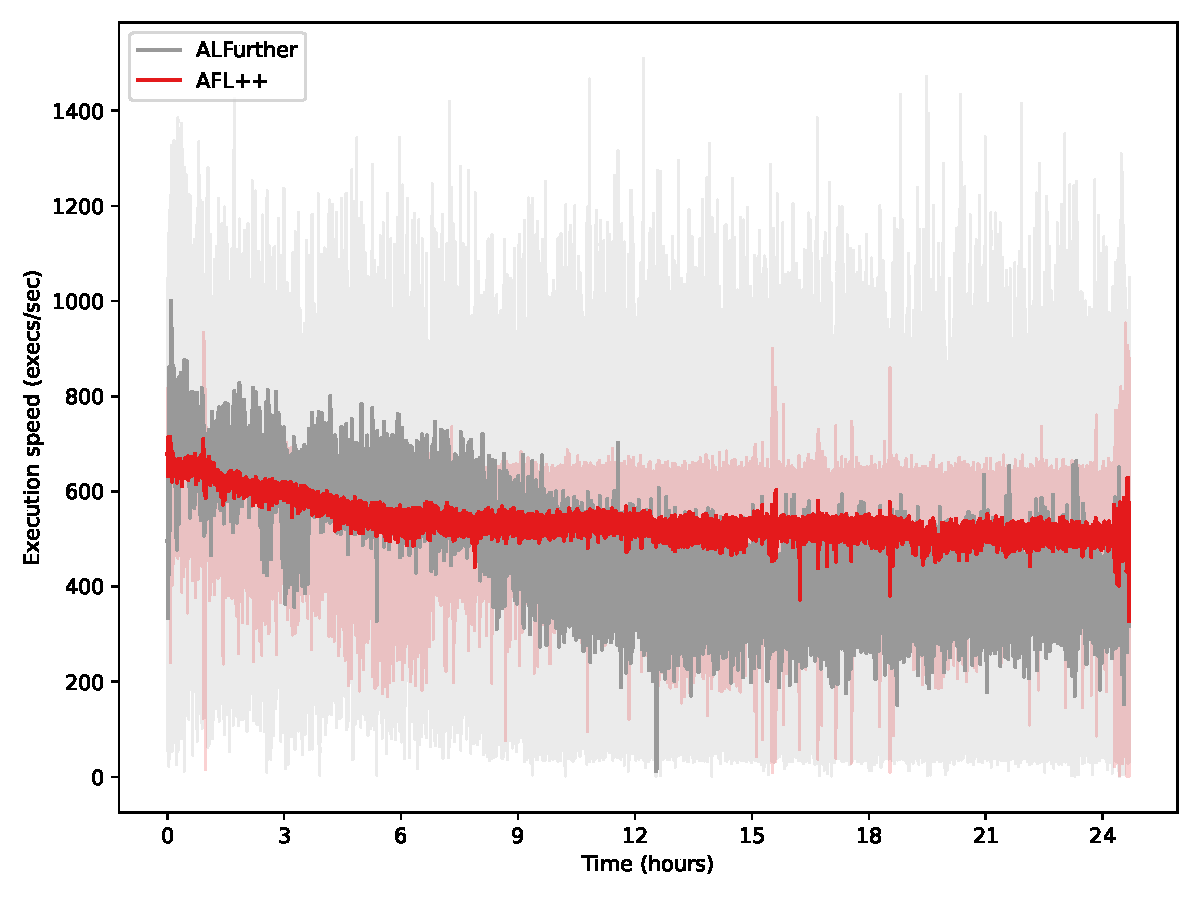
\includegraphics[width=0.25\textwidth]{results/ablation_study/overhead_infotocap.pdf}}
		\subfloat[\centering\normalsize mp3gain\label{fig:overhead-mp3gain}]{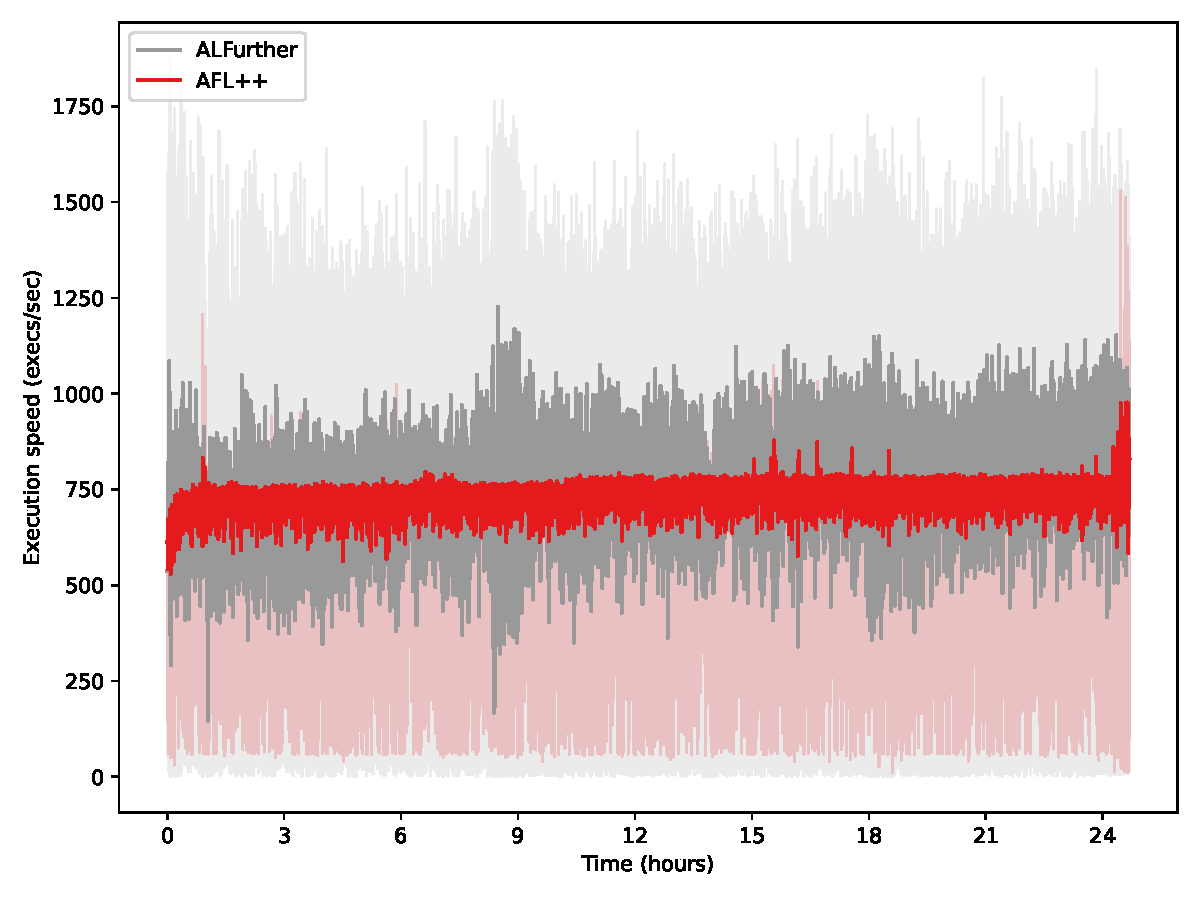
\includegraphics[width=0.25\textwidth]{results/ablation_study/overhead_imginfo.pdf}}
		\subfloat[\centering\normalsize pdftotext\label{fig:overhead-pdftotext}]{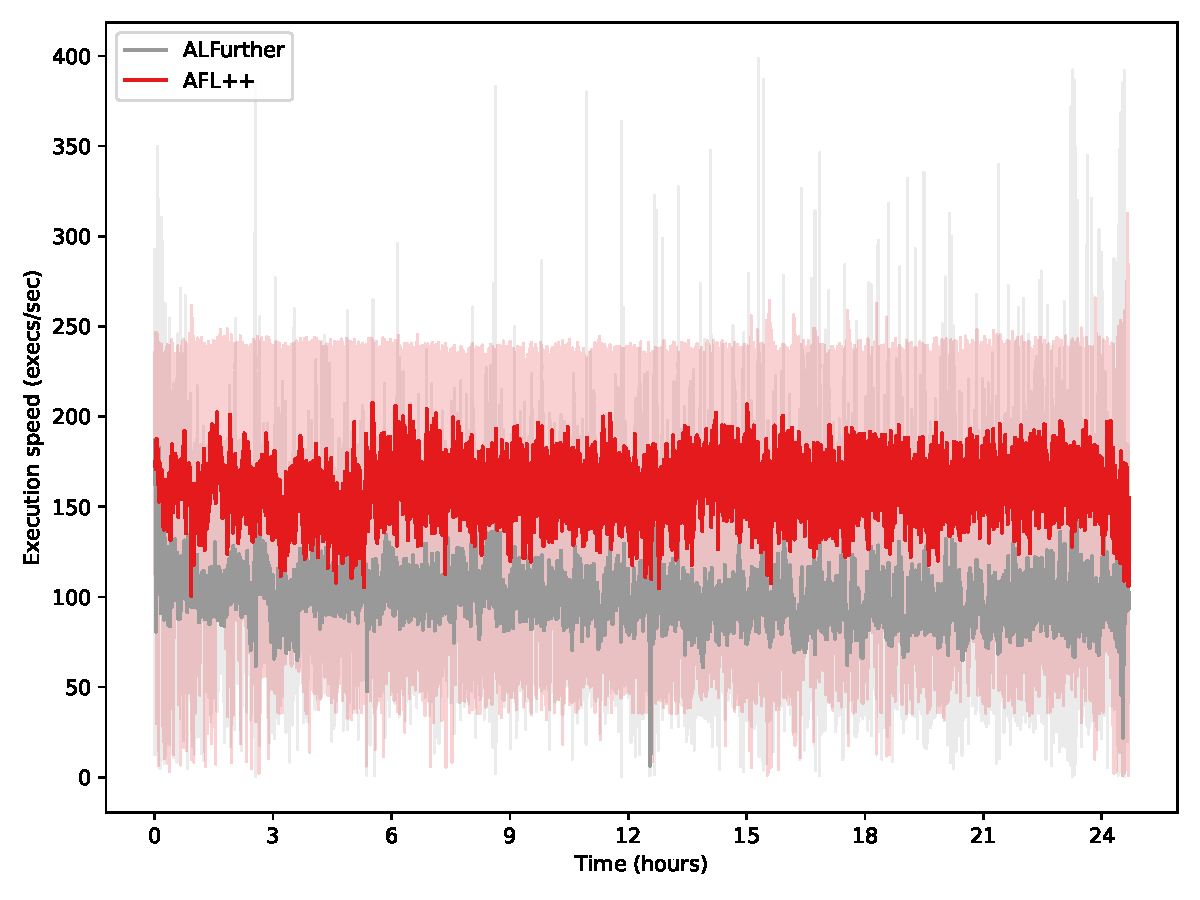
\includegraphics[width=0.25\textwidth]{results/ablation_study/overhead_pdftotext.pdf}}
		\subfloat[\centering\normalsize tiffsplit\label{fig:overhead-tiffsplit}]{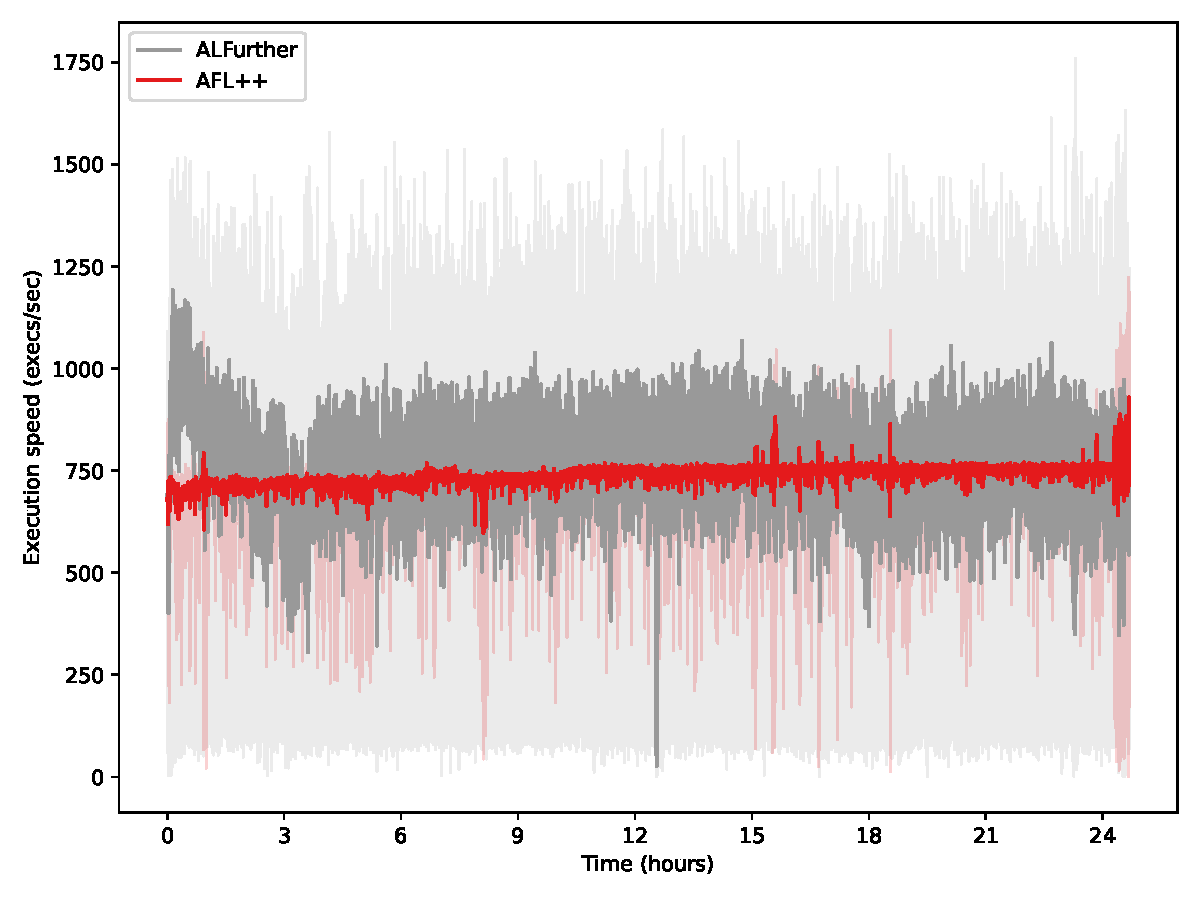
\includegraphics[width=0.25\textwidth]{results/ablation_study/overhead_tiffsplit.pdf}}
		%	}
	\caption{The executions per second of AFLplusplus and ALFruther over 24 hours and 5 runs.}
	\label{fig:overhead_plot}
\end{figure*}
\begin{figure*}[t!]
	%	\centerline{
		\subfloat[\centering\normalsize infotocap\label{fig:reward-infotocap}]{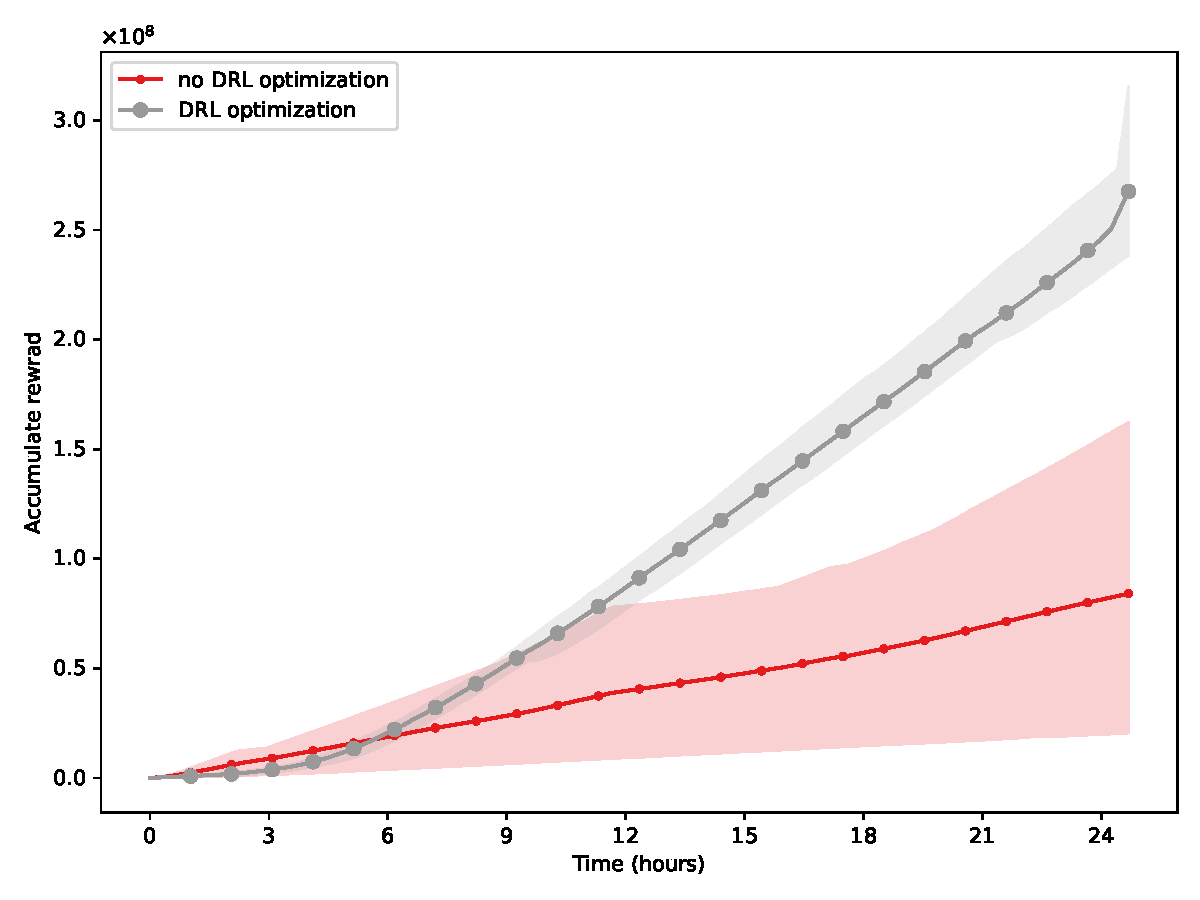
\includegraphics[width=0.25\textwidth]{results/ablation_study/reward_infotocap.pdf}}
		\subfloat[\centering\normalsize mp3gain\label{fig:reward-mp3gain}]{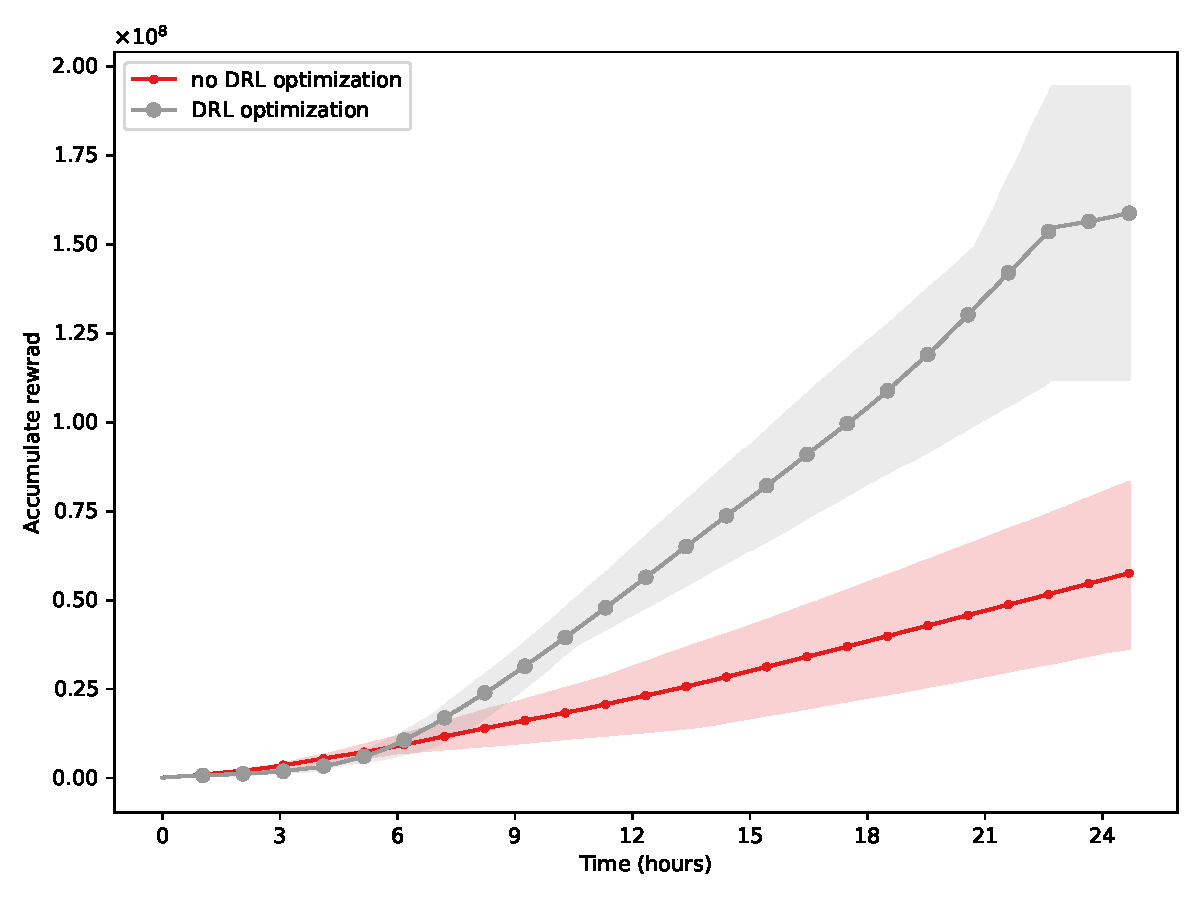
\includegraphics[width=0.25\textwidth]{results/ablation_study/reward_mp3gain.pdf}}
		\subfloat[\centering\normalsize pdftotext\label{fig:reward-pdftotext}]{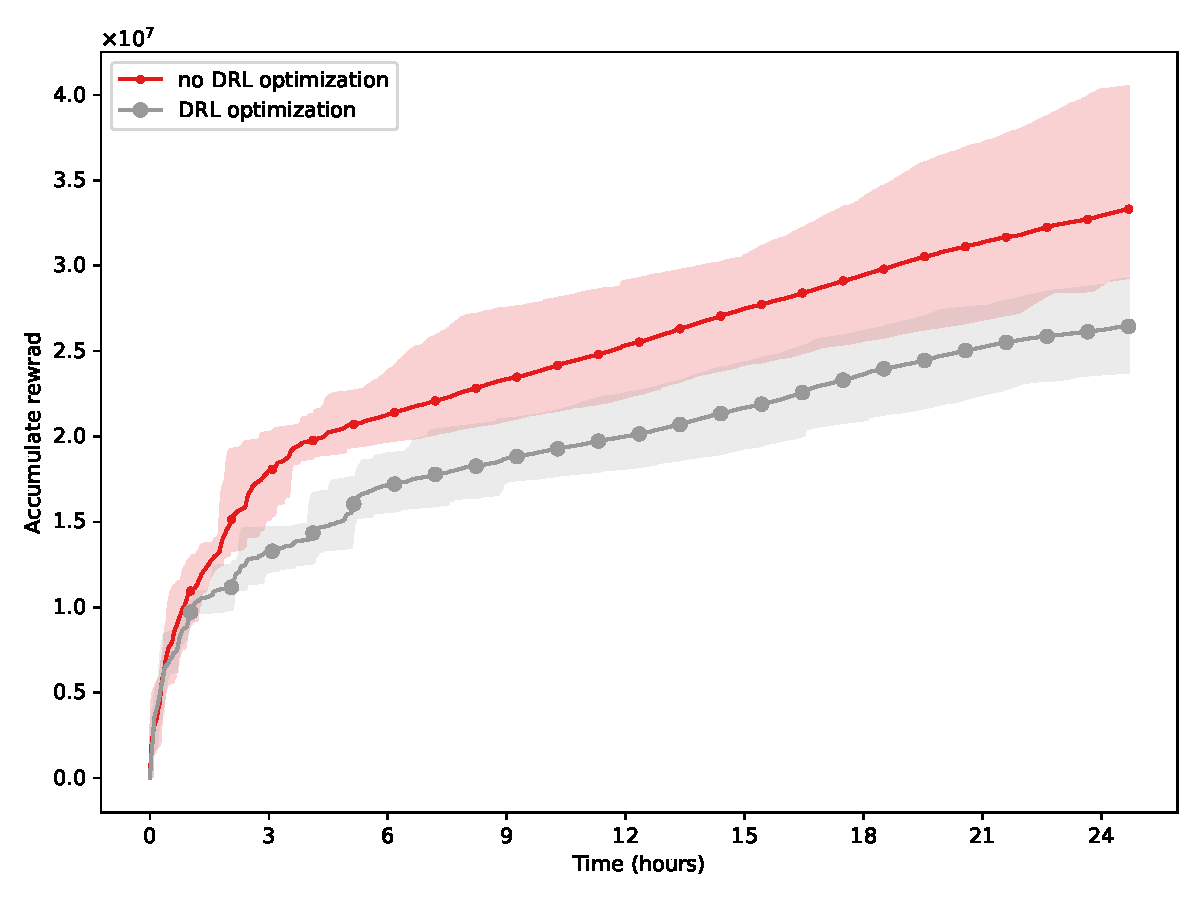
\includegraphics[width=0.25\textwidth]{results/ablation_study/reward_pdftotext.pdf}}
		\subfloat[\centering\normalsize tiffsplit\label{fig:reward-tiffsplit}]{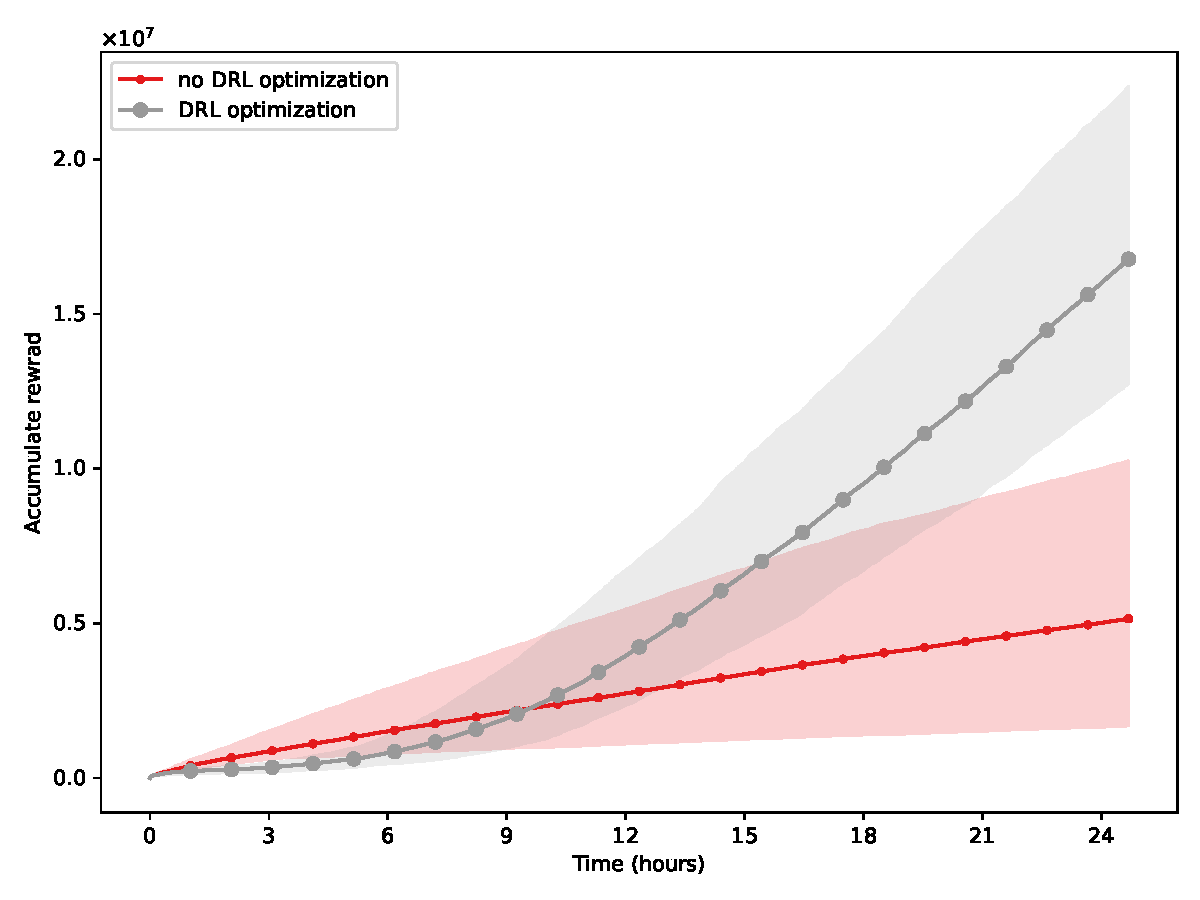
\includegraphics[width=0.25\textwidth]{results/ablation_study/reward_tiffsplit.pdf}}
		%	}
	\caption{The average accumulative rewards of AFLFurther with and without DRL optimizaiton and ALFruther over 24 hours and 5 runs.}
	\label{fig:reward_plot}
\end{figure*}

\subsubsection{Reward Analysis}\label{subsubsec:reward_analysis}

To assess the effectiveness of DRL-based optimization, we recorded the per-minute cumulative reward throughout each fuzzing campaign, with the reward defined as in Equation \ref{eq:reward}. Table \ref{tab:reward_analysis} summarizes the final cumulative rewards. Overall, DRL-optimized fuzzing achieves up to a 150\% higher cumulative reward than the non-optimized baseline, with the maximum observed improvement exceeding 220\%. These results validate the effectiveness of our DRL scheduler for the chosen objective function. Notably, in the case of \textit{pdftotext}, the DRL-guided approach yields an approximately 20\% lower reward than the baseline, indicating that the optimization does not yield consistent benefits across all targets; however, this performance reduction remains within an acceptable margin.

An additional noteworthy observation is that, despite the substantial reward improvement for \textit{mp3gain}, the corresponding edge coverage does not increase as expected (see Table \ref{tab:edge_coverage}). This discrepancy suggests that the current reward function may not sufficiently correlate with edge-coverage metrics. Thus, further research should explore alternative reward function designs to more directly incentivize coverage improvements in DRL-guided fuzzing.

Figure \ref{fig:reward_plot} depicts the cumulative reward curves over time. DRL-optimized fuzzing initially accrues lower rewards, likely reflecting an initial exploration or "warm-up" phase. As the campaign progresses, however, the DRL policy improves, ultimately achieving an exponential increase in cumulative reward relative to the baseline (i.e., fuzzing without DRL). The exception remains \textit{pdftotext}, where the cumulative reward consistently lags behind that of the non-DRL baseline, as reflected in Table \ref{tab:reward_analysis}. This finding aligns with the observation that ALFurther's code coverage on \textit{pdftotext} is also lower than that achieved by AFL++. These results suggest that, while DRL optimization is generally effective, its robustness across all targets is not yet assured—a limitation that warrants further investigation in future work.

\textbf{Answer to RQ4}: In most cases, DRL-based optimization substantially enhances cumulative reward according to the defined objective function. However, future work is needed to refine the reward function and improve the robustness of the approach across a broader range of targets.


% Table generated by Excel2LaTeX from sheet 'Reward'



\section{Discussion}
This section discusses key issues, limitations, and future directions that impact the applicability of ALFurther, providing insights for subsequent research.

\subsection{MDP Design}
As described in Section~\ref{subsec:mdp_construction}, our Markov Decision Process (MDP) construction is based on a selected set of common features, but there are several avenues for improvement:

\subsubsection{State Representation}
The state representation primarily utilizes byte-level features, including seed bytes and edge bitmaps. However, other features—such as execution time and fuzzing depth—have demonstrated effectiveness in related studies~\cite{binosiRainfuzzReinforcementlearningDriven2023, linDeepGoPredictiveDirected2024}. Our approach models these features as sparse images and employs visualization techniques to learn latent representations, which may inadvertently diminish the informational content of certain discrete features. Future work could explore integrating additional features and alternative state abstractions to enrich the environmental representation.

\subsubsection{Action Space}
Similar to the state design, our current approach emphasizes continuous fuzzing strategies. In contrast, several studies have adopted discrete action spaces, such as selecting specific mutation locations or mutator types~\cite{bottingerDeepReinforcementFuzzing2018, liangRLFDirectedFuzzing2022}. We favor continuous strategies because they offer prolonged guidance during fuzzing and reduce the need for frequent interaction with the DRL model. In contrast, discrete strategies may require model inference at every fuzzing step, increasing computational overhead. Moreover, continuous policies preserve exploration, since actions are sampled from a policy distribution, introducing beneficial randomness. However, deterministic or discrete actions can have a stronger influence and may be more effective as models approach optimality. Thus, investigating DRL-based fuzzing optimization using deterministic actions with low overhead and high explorability remains a promising direction.

\subsection{Reward Function}
As outlined in Section~\ref{subsubsec:reward}, our reward function is designed to balance global edge coverage gains with local changes. However, empirical results reveal that this formulation lacks robustness across diverse fuzzing targets, sometimes leading to misalignment between reward signals and actual coverage improvements, and occasionally resulting in suboptimal cumulative rewards, as discussed in Section~\ref{subsubsec:reward_analysis}. While our primary aim was to demonstrate the feasibility of applying DRL to coverage-guided fuzzing (CGF)—which is supported by extensive experimental results—the current reward function remains “adequate” rather than “optimal.” These findings underscore the critical importance of refining reward function design for DRL-based fuzzing and highlight it as an essential area for future research.

Furthermore, as detailed in Section~\ref{subsubsec:magma_analysis}, the reward function may lack sufficient adaptability for bug discovery tasks. Insights from MOPT~\cite{lyuMOPTOptimizedMutation2019} indicate that incorporating metrics tied directly to crash discovery efficiency could further enhance bug-finding performance. However, such integration would significantly increase implementation complexity, which is beyond the scope of this work, but it represents an important direction for future investigation.

\subsection{DRL Training Methodology}
Our approach employs an offline, model-free DRL algorithm (SAC) to accommodate the asynchronous execution patterns of coverage-guided fuzzing, effectively addressing sample utilization and training efficiency. Alternatively, model-based DRL techniques, such as MuZero~\cite{schrittwieserMasteringAtariGo2020}, could decouple optimization from exploration and improve sample efficiency. However, these approaches demand accurate environment modeling for policy evaluation, which introduces substantial implementation challenges for CGF. Future research could explore model-based DRL as advances in fuzzing environments and modeling mature.

\subsection{Practical Considerations and External Validity}
ALFurther’s implementation introduces several practical challenges, primarily related to hardware and benchmarking environments.

\subsubsection{GPU Support}
Our DRL implementation leverages a ResNet-based observer for learning state representations, necessitating GPU resources for efficient model training. In contrast, traditional fuzzing frameworks typically require only CPU resources, raising concerns regarding deployment scalability. 

Nevertheless, with the increasing role of artificial intelligence in program analysis and bug discovery, GPU requirements are likely to become more acceptable. A promising direction is to adopt a client-server architecture: CPU-based edge devices could execute fuzzing while centralized GPU servers handle training and policy updates. Using a single model to serve multiple fuzzing processes, our emulation of this design demonstrated increased effectiveness by leveraging larger sample pools. While this emulation is not the central focus of our study, the approach is relevant for practical deployment scenarios.

\subsubsection{Disk I/O and Storage Requirements}
Another limitation involves disk I/O performance and storage capacity. Communication between fuzzers and models relies on file-based IPC, which requires high disk I/O throughput to minimize communication overhead. In our evaluation, solid-state drives effectively mitigated this issue, but systems with slower disks may experience higher latency. Additionally, our MDP buffer—set to a capacity of 100,000—requires approximately 30 GB of disk space. In-memory mounting could alleviate storage demands but necessitates large amounts of available RAM. Reducing the number of stored samples or improving training efficiency to decrease buffer size are important topics for future work and improving framework deployability.

\subsubsection{Benchmark Selection}
To ensure a fair and consistent evaluation protocol, we utilized two widely adopted public benchmarks—UniBench and MAGMA. We did not employ FuzzBench~\cite{metzmanFuzzBenchOpenFuzzer2021} due to its complex, multi-stage workflow, which complicates adaptation for GPU-supported DRL training. Future work may extend the evaluation to FuzzBench as GPU-compatible adaptations become available, further enhancing the comprehensiveness and generalizability of our results.

\subsubsection{Discovery of Unknown Bugs}
This study did not prioritize discovering previously unknown bugs, a common metric in prior fuzzing research. Ongoing large-scale bug discovery efforts by OSS-Fuzz~\cite{aryaOSSfuzz2025} make identifying new bugs in well-tested software increasingly difficult. Instead, we argue that comparative benchmarking under consistent protocols yields a more reliable assessment of fuzzer effectiveness than the resource-intensive pursuit of novel bugs in less-studied programs. Nonetheless, we plan to continue testing ALFurther on diverse software targets and will report any new crashes to relevant developers.


\section{Related Work}\label{sec:related_work}
%	\subsection{Optimization-based Fuzzing}
This work investigates the optimization of fuzzing based on DRL techniques. Accordingly, the related work is organized into two main themes: fuzzing optimization techniques and DRL-based fuzzing approaches.
\subsection{Optimization Techniques in Fuzzing}
Various optimization techniques have been proposed to enhance the performance of coverage‑guided fuzzing (CGF) by selecting fuzzing strategies. The methods mainly include optimizing specific problems, and the general optimization based on adaptive methods.

\subsubsection{Optimization to Specific Problem}
Many works address particular challenges in fuzzing by applying statistical analyses to guide the scheduling of testcases. For example, FairFuzz \cite{lemieuxFairFuzzTargetedMutation2018} targets the exploration problem on rarely visited branches and introduces a byte‐level, branch-specific scheduling scheme to guide fuzzing toward those hard‐to‐reach targets. Entropic \cite{bohmeBoostingFuzzerEfficiency2020} introduces an entropy‐driven scheduler that devotes more resources to seeds with higher information gain, thereby stimulating path exploration. EMS \cite{lyuEMSHistorydrivenMutation2022} leverages historical fuzzing records to identify and reuse effective mutation operators from past executions, improving performance on target programs relevant to the past test. Alphuzz \cite{zhaoAlphuzzMonteCarlo2022} addresses the issue that existing scheduling approaches overlook the dependency relationships among testcases. It formulates seed selection as a Monte Carlo Tree Search problem, scheduling testcases based on the expected optimal paths within the mutation tree. Although these approaches demonstrate their effectiveness under the intended conditions, they have limited versatility in diverse general-purpose fuzzing scenarios, thereby restricting their performance across various testing environments.

\subsubsection{General Optimization}
For greater generality and adaptability, several studies have introduced heuristic search algorithms to optimize fuzzing strategies. For example, MOPT \cite{lyuMOPTOptimizedMutation2019} applies a particle swarm optimization algorithm to evaluate the reward of each mutation strategy and select the most promising one. DARWIN \cite{jauernigDARWINSurvivalFittest2023} follows the insights of MOPT and explores the mutation strategies with perturbation to generate new best-performing candidates based on the evolution algorithm. However, heuristic optimization relies heavily on exhaustive state space exploration \cite{russellArtificialIntelligenceModern2020}, which may incur substantial computational overhead. Moreover, heuristics typically yield only feasible (but not necessarily optimal) solutions, offering no guarantee of global optimality \cite{hartFormalBasisHeuristic1968}. As a result, the optimal strategy under a state may be overlooked, and the overall effectiveness of the optimization may remain limited.

Inspired by Reinforcement Learning (RL), several studies employ Multi-armed Bandit (MAB) algorithms to optimize fuzzing strategies. For instance, EcoFuzz \cite{yueEcoFuzzAdaptiveEnergysaving2020} formulates fuzzing as a Markov Chain and applies an MAB algorithm for seed scheduling optimization to maximize the discovery of new execution paths. BeliefFuzz \cite{huangBalanceSeedScheduling2023} models fuzzing as a Monte Carlo process and adopts the Upper Confidence Bound algorithm to select seeds that offer the highest expected path‑discovery potential at minimal cost. Likewise, SeamFuzz \cite{leeLearningSeedadaptiveMutation2023} frames seed scheduling as a multi-armed bandit problem, employing Thompson sampling to schedule the seeds with similar characteristics. These studies demonstrate the promise of applying reinforcement‑learning techniques to fuzzing optimization. However, conventional RL methods—such as multi‑armed bandits—are inherently constrained by their simplistic representations of the environment, with limited state and action modeling capacity. Therefore, these approaches often struggle to approximate complex environments and effectively predict optimal policies, limiting the effectiveness of the approaches across diverse scenarios. As a result, it underscores the need to develop more comprehensive RL frameworks in fuzzing applications.

\subsection{DRL-based Fuzzing}
DRL techniques employ an NN model for the modeling, estimation, and policing, which significantly improves the capability of complex environment modeling and the effectiveness of policy optimization. Existing work in DRL‑based fuzzing can be divided into domain‑specific approaches, which aim for particular classes of targets, and general‑purpose methods that tailor the optimization across diverse programs.

\subsubsection{Domain-specific Fuzzing}

Recent studies in domain-specific fuzzing primarily target the application domains with well-defined input structures, particularly language-specific targets benefiting from advances in Large Language Models (LLMs). The integration of LLMs and DRL-based fuzzing has experienced significant growth, with techniques typically involving fine-tuning pretrained models using DRL to guide semantic mutation, particularly token selection to generate structured inputs. For instance, CovRL \cite{eomFuzzingJavaScriptInterpreters2024} combines an LLM with DRL methodologies to perform semantic mutations specifically tailored for JavaScript interpreter fuzzing. Similarly, BertRLFuzzer \cite{jhaBertRLFuzzerBERTReinforcement2024} utilizes the PPO algorithm \cite{schulmanProximalPolicyOptimization2017} to fine-tune the BERT model \cite{devlinBERTPretrainingDeep2019}, enabling effective generation of semantic testcases for web application fuzzing.

On the other hand, most domain-specific DRL fuzzing studies assume an explicit structure of grammar and syntax, thus limiting the mutation action space to semantic tokens. However, such methods encounter challenges when confronted with input data represented as byte streams, which lack clear structural definitions. Consequently, developing DRL-based fuzzing optimization to handle general-purpose, unstructured input mutation remains a crucial and promising avenue for future research.

\subsubsection{General Fuzzing}
The development of general‑purpose DRL fuzzing has proceeded more slowly. This slower progress can be attributed to three main challenges: first, the considerable engineering effort required to integrate DRL agents into existing fuzzing implementations; second, the difficulty in adapting DRL workflows to generic fuzzing processes; and last, the substantial state and action spaces encountered in general fuzzing, which impose demands on efficient exploration and policy optimization.

Among existing studies, Deep Reinforcement Fuzzing \cite{bottingerDeepReinforcementFuzzing2018} may be one of the pioneering efforts employing empirical exploration in general fuzzing. It utilizes a DQN model to identify the mutation positions of testcases and demonstrates feasibility through preliminary evaluations. Similarly, RLF \cite{liangRLFDirectedFuzzing2022} adopts a DQN-based model to determine whether to skip the current testcase, enhancing the performance of directed fuzzing. Also, RainFuzz \cite{binosiRainfuzzReinforcementlearningDriven2023} leverages the PPO algorithm to predict mutation positions and mutation operators.

Although these studies demonstrate the potential of DRL in fuzzing optimization, they lack a formalized definition of DRL-based fuzzing problems and explicit structuring of the necessary components. This absence of formalization limits clarity regarding feasibility and hinders further advancement. Moreover, these approaches primarily focus on specific fuzzing operations and do not consider the optimization of more comprehensive fuzzing strategies. Additionally, their empirical experiments are typically conducted on ad hoc, private benchmarks, which lack consistency in evaluation standards \cite{kleesEvaluatingFuzzTesting2018}. Some attempts on evaluation standardization, such as the development of DRL-specific simulated environments \cite{drozdFuzzerGymCompetitiveFramework2018}, also diverge significantly from real-world fuzzing scenarios. Consequently, the DRL-based CGF methodologies have not been evaluated against extensive public benchmarks, constraining DRL-based fuzzing optimizations' reliability and broader applicability.

To overcome these limitations, our study formalizes the objectives of CGF and theoretically demonstrates the feasibility of optimizing CGF strategies through DRL techniques. Besides, we construct a prototype based on the formalization, explicitly defining each component of a DRL fuzzing framework. Furthermore, we implement various strategies to ensure compatibility and seamless integration between the DRL framework and conventional fuzzers. Finally, we conduct rigorous evaluations of our prototype on two prominent public fuzzing benchmarks, thoroughly verifying the effectiveness of DRL-based CGF optimization through diverse experimental scenarios and analytical assessments.

Among the related DRL-based fuzzing studies, DeepGo \cite{linDeepGoPredictiveDirected2024} shares certain similarities with our work. Both approaches utilize the SAC \cite{haarnojaSoftActorcriticOffpolicy2018} algorithm and incorporate action design to optimize scheduling strategies. However, DeepGo targets directed fuzzing, employing trajectory as states that reflect seed path transitions. In contrast, our method addresses general coverage-guided fuzzing and captures discrete information for individual samples rather than their sequential trajectories, better aligning with CGF's asynchronous features. Additionally, our reward structure differs significantly: DeepGo prioritizes reaching specific targets, whereas our approach emphasizes maximizing code coverage. In summary, our study contributes mainly to optimizing CGF through DRL by providing theoretical grounding, a structured framework, and insights from practical implementation, potentially serving as a bedrock for future research.

\section{Conclusion}\label{sec:conclusion}

This paper investigates the theoretical and practical feasibility of using DRL techniques to optimize fuzzing strategies under real scenarios. Specifically, we formally define the objective of coverage-guided fuzzing and demonstrate the theoretical viability of employing DRL techniques for optimizing fuzzing strategies. Building upon the above foundation, we propose ALFurther, a prototype that implements the essential components of the MDP, integrates a comprehensive DRL framework, and develops strategies compatible with existing fuzzing processes.	To validate the effectiveness of DRL-based fuzzing optimization under real fuzzing scenarios, we evaluate ALFurther using two publicly available benchmarks, Unibench and MAGMA. Experimental results indicate that ALFurther significantly surpasses several existing optimization-based fuzzers in terms of both code coverage and bug discovery efficiency.

The implementation and evaluation results in the study could also provide insights for future research on DRL-driven fuzzing techniques. For example, future work could focus on refining the design of the MDP components to enhance bug discovery capabilities further. Also, developing seamless integration between fuzzers and DRL frameworks may help minimize overhead from inter-module communication and sample processing, improving fuzzing performance.

\bibliographystyle{IEEEtran}
\bibliography{ref.bib}




\vfill

\end{document}


